% =============================================================================
% Meta-Prediction Theory: A Complete Paper
% Target Journal: Psychological Review or Psychological Bulletin
% Format: Double-column, journal style
% =============================================================================

\documentclass[10pt,twocolumn]{article}
\usepackage[utf8]{inputenc}
\usepackage[T1]{fontenc}
\usepackage{amsmath,amssymb}
\usepackage{booktabs}
\usepackage{graphicx}
\usepackage{natbib}
\usepackage[margin=0.75in]{geometry}
\usepackage{setspace}
\usepackage{caption}
\usepackage{enumitem}
\usepackage{url}
\usepackage[colorlinks=true,linkcolor=blue,citecolor=blue,urlcolor=blue]{hyperref}

% Column separation
\setlength{\columnsep}{0.3in}

% Single spacing for double-column format
\singlespacing

% Caption formatting
\captionsetup{font=small,labelfont=bf}

% Compact lists
\setlist{nosep,leftmargin=*}

% =============================================================================
% TITLE (spans both columns)
% =============================================================================

\title{The Meta-Prediction Theory: A Recursive Meta-Cognitive Framework for Understanding Self-Report Bias in Psychological Assessment}
\author{Ziheng Zhou\\\texttt{leozhou201204@163.com}}
\date{}

\begin{document}
\maketitle

\begin{abstract}
\noindent Self-report measures, despite their ubiquity in psychological research and clinical assessment, suffer from a fundamental vulnerability: respondents can deliberately manipulate their responses to produce desired outcomes. We introduce the Meta-Prediction Theory, a novel theoretical framework that reconceptualizes self-report bias as a recursive meta-cognitive process. Rather than passively distorting responses based on social desirability, respondents actively predict what scales measure, anticipate how their responses will be interpreted, and strategically adjust their answers accordingly---a process that operates across multiple levels of prediction. We extend the traditional Three-Layer Meta-Cognitive Model by incorporating scale cognition and meta-prediction as additional components, deriving 15 testable propositions concerning the nature, determinants, and consequences of meta-prediction bias. An exploratory empirical analysis using a large-scale dataset ($N = 24{,}292$) provides preliminary support for our theoretical predictions: response time patterns are correlated with scale scores ($r = -.132$), the Deliberation proxy (inverse extreme responding) is the strongest meta-cognitive predictor (sr$^2 = .164$), and response time variables account for a meaningful portion of shared variance between depression and anxiety measures. The No-SA hierarchical regression model demonstrates superior fit to the data compared to alternative models (AIC $= 94{,}096$ vs.\ $111{,}131$ and $132{,}614$; $\Delta R^2 = .208$ over the concurrent-validity baseline). However, these findings must be interpreted with caution: the proxy variables are imperfect measures of meta-cognitive processes, and the observed patterns may reflect clinical comorbidity, floor effects, or fatigue rather than meta-prediction. This work represents a proof of concept for response time-based detection of meta-cognitive processes in self-report assessment. All findings are exploratory and require replication with external validation.

\medskip
\noindent\textbf{Keywords:} meta-prediction; social desirability bias; self-report bias; meta-cognition; psychological assessment; meta-cognitive processes; response time analysis
\end{abstract}

% =============================================================================
% INTRODUCTION
% =============================================================================

\section{Introduction}

Self-report measures are the backbone of psychological research and clinical assessment. From personality inventories to clinical screening instruments, researchers and clinicians rely heavily on individuals' self-reported experiences, attitudes, and behaviors. Yet beneath this reliance lies a persistent and troubling vulnerability: respondents can deliberately manipulate their responses to produce desired outcomes \citep{Paulhus1984}.

Consider, for example, a patient completing a depression screening questionnaire. This individual may wish to appear more depressed than they actually are---perhaps to secure treatment, elicit sympathy, or validate a self-diagnosis. Alternatively, they may wish to appear less depressed---to avoid stigma, prevent a psychiatric diagnosis, or maintain employment. In either scenario, the patient is not passively reporting their symptoms; they are actively engaged in a sophisticated cognitive process of predicting what the questionnaire measures and strategically adjusting their answers to achieve a desired outcome.

This phenomenon extends far beyond clinical assessment. In organizational psychology, job applicants routinely present themselves as more conscientious, agreeable, and emotionally stable than their actual dispositions would suggest. In educational research, students may overreport their motivation, engagement, and study habits. In health psychology, patients systematically overreport healthy behaviors (exercise, diet) while underreporting unhealthy ones (substance use, sedentary behavior).

The dominant paradigm for addressing this question has focused on \textit{social desirability bias}---the tendency to present oneself in a favorable light \citep{Edwards1953, CrowneMarlowe1960}. Paulhus's \citep{Paulhus1984} influential Two-Component Model distinguishes between \textit{Self-Deceptive Enhancement} (SDE; honest but positively biased self-reports) and \textit{Impression Management} (IM; deliberate self-presentation to an audience). While this framework has proven invaluable, it suffers from several critical limitations.

First, existing models treat social desirability as a \textit{stable trait}, ignoring the \textit{dynamic processes} that generate bias in specific assessment contexts. Second, these models fail to account for the \textit{recursive nature} of meta-prediction. Respondents do not simply decide to present themselves favorably; they engage in multi-level predictions about what the scale expects, how their responses will be interpreted, and what answers will produce the desired impression. Third, existing models provide no mechanism for explaining \textit{how} bias occurs. Fourth, they ignore the role of \textit{scale literacy}---respondents' knowledge of psychological constructs and assessment methods---in shaping their responses.

This paper introduces the \textit{Meta-Prediction Theory}, a novel theoretical framework that addresses these limitations. The theory makes five key contributions:

\begin{enumerate}
    \item \textbf{Recursive Meta-Prediction}: The theory introduces the concept of recursive meta-prediction, where respondents predict what scales expect at multiple levels (first-order: ``What is being measured?''; second-order: ``What answer is expected?''; third-order: ``How should I adjust my response?'').
    \item \textbf{Scale Cognition}: The theory introduces Scale Cognition as a distinct construct, representing respondents' awareness of psychological constructs and their understanding of how scales operate.
    \item \textbf{Response Time Integration}: The theory integrates response time data as an objective, non-self-report measure of meta-cognitive processes.
    \item \textbf{Cross-Scale Consistency}: The theory introduces a regression-based approach to adjusting for cross-scale consistency, which accounts for meta-cognitive processes in self-report measures.
    \item \textbf{Computational Modeling}: The theory provides a computational model that simulates meta-prediction processes and generates testable predictions.
\end{enumerate}

% =============================================================================
% THEORETICAL BACKGROUND
% =============================================================================

\section{Theoretical Background}

\subsection{Social Desirability Bias: A Historical Overview}

Research on social desirability bias has a long history in psychology. Edwards \citep{Edwards1953} first introduced the concept of social desirability in personality assessment. Crowne and Marlowe \citep{CrowneMarlowe1960} developed the Marlowe-Crowne Social Desirability Scale (MC-SDS), which has become the most widely used measure of social desirability bias. Subsequent work has identified distinct response styles, including acquiescence, extremity, and midpoint responding \citep{Baumgartner2001, Weijters2010}, as well as the role of test-taking motivation in shaping response quality \citep{Krosnick1991, Wise2006}. Careless and insufficient effortful responding has been identified as a major threat to data quality, with extreme responding and rapid completion serving as key indicators \citep{Meade2012}. Cross-cultural research has examined how social desirability and response styles manifest in non-Western populations \citep{Huang2012}, which is particularly relevant given that the present study uses a Chinese sample.

Paulhus \citep{Paulhus1984} advanced the field by proposing the Two-Component Model, which distinguishes between two forms of socially desirable responding:

\begin{enumerate}
    \item \textbf{Self-Deceptive Enhancement (SDE)}: The tendency to give self-reports that are honest but positively biased. This is an unconscious process where individuals genuinely believe their overly positive self-descriptions.
    \item \textbf{Impression Management (IM)}: The tendency to deliberately present oneself favorably to an audience. This is a conscious process involving strategic self-presentation.
\end{enumerate}

While Paulhus's model has been influential, it has several limitations: it treats social desirability as a stable trait, ignoring dynamic processes; it does not account for the recursive nature of meta-prediction; it does not explain the cognitive mechanisms underlying bias; and it does not consider how respondents' knowledge of psychological constructs affects their responses.

\subsection{Meta-Cognition and Self-Report}

Meta-cognition refers to the ability to monitor and regulate one's own cognitive processes \citep{Flavell1979}. In the context of self-report, meta-cognition involves meta-cognitive monitoring (awareness of one's own thoughts, feelings, and behaviors) and meta-cognitive regulation (the ability to control and adjust one's responses based on this awareness). Recent research has shown that meta-cognitive processes play a significant role in self-report \citep{Paulhus2002}, but their role in social desirability bias has not been fully explored. Importantly, the concept of ``scale cognition'' overlaps with existing constructs such as test-taking skills \citep{Goffin2003}, item cueing \citep{McFarland2000}, and impression management in high-stakes contexts \citep{Griffith2007}. The present work aims to integrate these perspectives under a unified meta-cognitive framework.

\subsection{Computational Approaches to Response Processes}

Recent advances in computational modeling have provided new tools for understanding response processes. Evidence accumulation models, such as the Drift Diffusion Model (DDM), have been successfully applied to response time data in cognitive tasks \citep{Ratcliff1978, Ratcliff2008} and, more recently, to survey responding \citep{Vandekerckhove2007}. These models conceptualize responding as a process of evidence accumulation toward a decision threshold, with response time reflecting the speed of this process. The Meta-Prediction Theory extends this framework by proposing that the evidence accumulation process is influenced by meta-cognitive predictions about what the scale expects.

\subsection{The Meta-Prediction Theory}

The Meta-Prediction Theory proposes that self-report bias arises from a recursive meta-cognitive process in which respondents predict what a scale is measuring and adjust their answers accordingly. The theory includes five key components:

\begin{enumerate}
    \item \textbf{Actual Self-Cognition (ASC)}: Awareness of one's true feelings, behaviors, and attitudes.
    \item \textbf{Desired Self-Cognition (DSC)}: Awareness of one's ideal self and personal standards.
    \item \textbf{Social Desirability Cognition (SDC)}: Awareness of social norms and expectations.
    \item \textbf{Meta-Cognitive Monitoring (MCM)}: The ability to detect discrepancies between actual and desired states.
    \item \textbf{Meta-Cognitive Regulation (MCR)}: The tendency to adjust answers based on social expectations.
\end{enumerate}

The theory also introduces the concept of \textbf{Scale Cognition}---the awareness of what the scale is measuring and how responses will be interpreted. This is distinct from self-deception and impression management, as it involves a meta-cognitive process of predicting the scale's expectations.

% =============================================================================
% THE META-PREDICTION MODEL
% =============================================================================

\section{The Meta-Prediction Model}

\subsection{Model Overview}

The Meta-Prediction Model describes the process by which respondents generate desired answers through recursive meta-cognitive processes. The model includes five key parameters:

\begin{enumerate}
    \item \textbf{Memory Accuracy ($\alpha$)}: Accuracy of recalling actual experiences
    \item \textbf{Self-Awareness ($\sigma$)}: Clarity of self-perception
    \item \textbf{Ideal Self-Strength ($\delta$)}: Strength of ideal self-concept
    \item \textbf{Norm Awareness ($\nu$)}: Awareness of social expectations
    \item \textbf{Meta-Cognitive Capacity ($\mu$)}: Ability to monitor and regulate responses
\end{enumerate}

\subsection{Model Equations}

The model can be formalized as follows:
\begin{equation}
R = f(S, D, M, P)
\end{equation}
where $R$ is the reported answer, $S$ is the true state (actual self-cognition), $D$ is the desired state (desired self-cognition), $M$ is meta-cognitive monitoring (awareness of discrepancy), and $P$ is meta-prediction (prediction of scale expectations).

The meta-prediction component $P$ is recursive and can be formalized using a Bayesian updating framework. At each prediction level $i$, the respondent updates their belief about the scale's expectations based on prior beliefs and observed evidence:
\begin{equation}
P_i = \frac{P(e|H_i) \cdot P(H_i)}{P(e)}
\end{equation}
where $P(H_i)$ is the prior probability of hypothesis $H_i$ (e.g., ``the scale measures depression''), $P(e|H_i)$ is the likelihood of observing evidence $e$ (e.g., item content, response options) given $H_i$, and $P(e)$ is the marginal probability of the evidence. The recursive process terminates when the respondent reaches a sufficiently confident prediction or when cognitive resources are exhausted \citep{Ratcliff1978}.

Alternatively, the recursive process can be modeled as a hierarchical evidence accumulation process:
\begin{equation}
\frac{dP_i}{dt} = \delta_i + \sigma \cdot W(t)
\end{equation}
where $\delta_i$ is the drift rate (speed of evidence accumulation at level $i$), $\sigma$ is noise, and $W(t)$ is a Wiener process. This formulation connects the Meta-Prediction Theory to established computational frameworks in cognitive science \citep{Ratcliff2008, Vandekerckhove2007}.

\subsection{Computational Implementation}

The model was implemented in Python (see Figure~\ref{fig:model_diagram} for the model diagram). The implementation follows a layered architecture where each cognitive component (Actual Self, Desired Self, Social Desirability, Scale Cognition, Meta-Cognitive Monitoring, Meta-Cognitive Regulation) feeds into the final desired answer through recursive meta-prediction processes.

% =============================================================================
% FIGURE 1: Model Diagram
% =============================================================================

\begin{figure}[tbp]
\centering
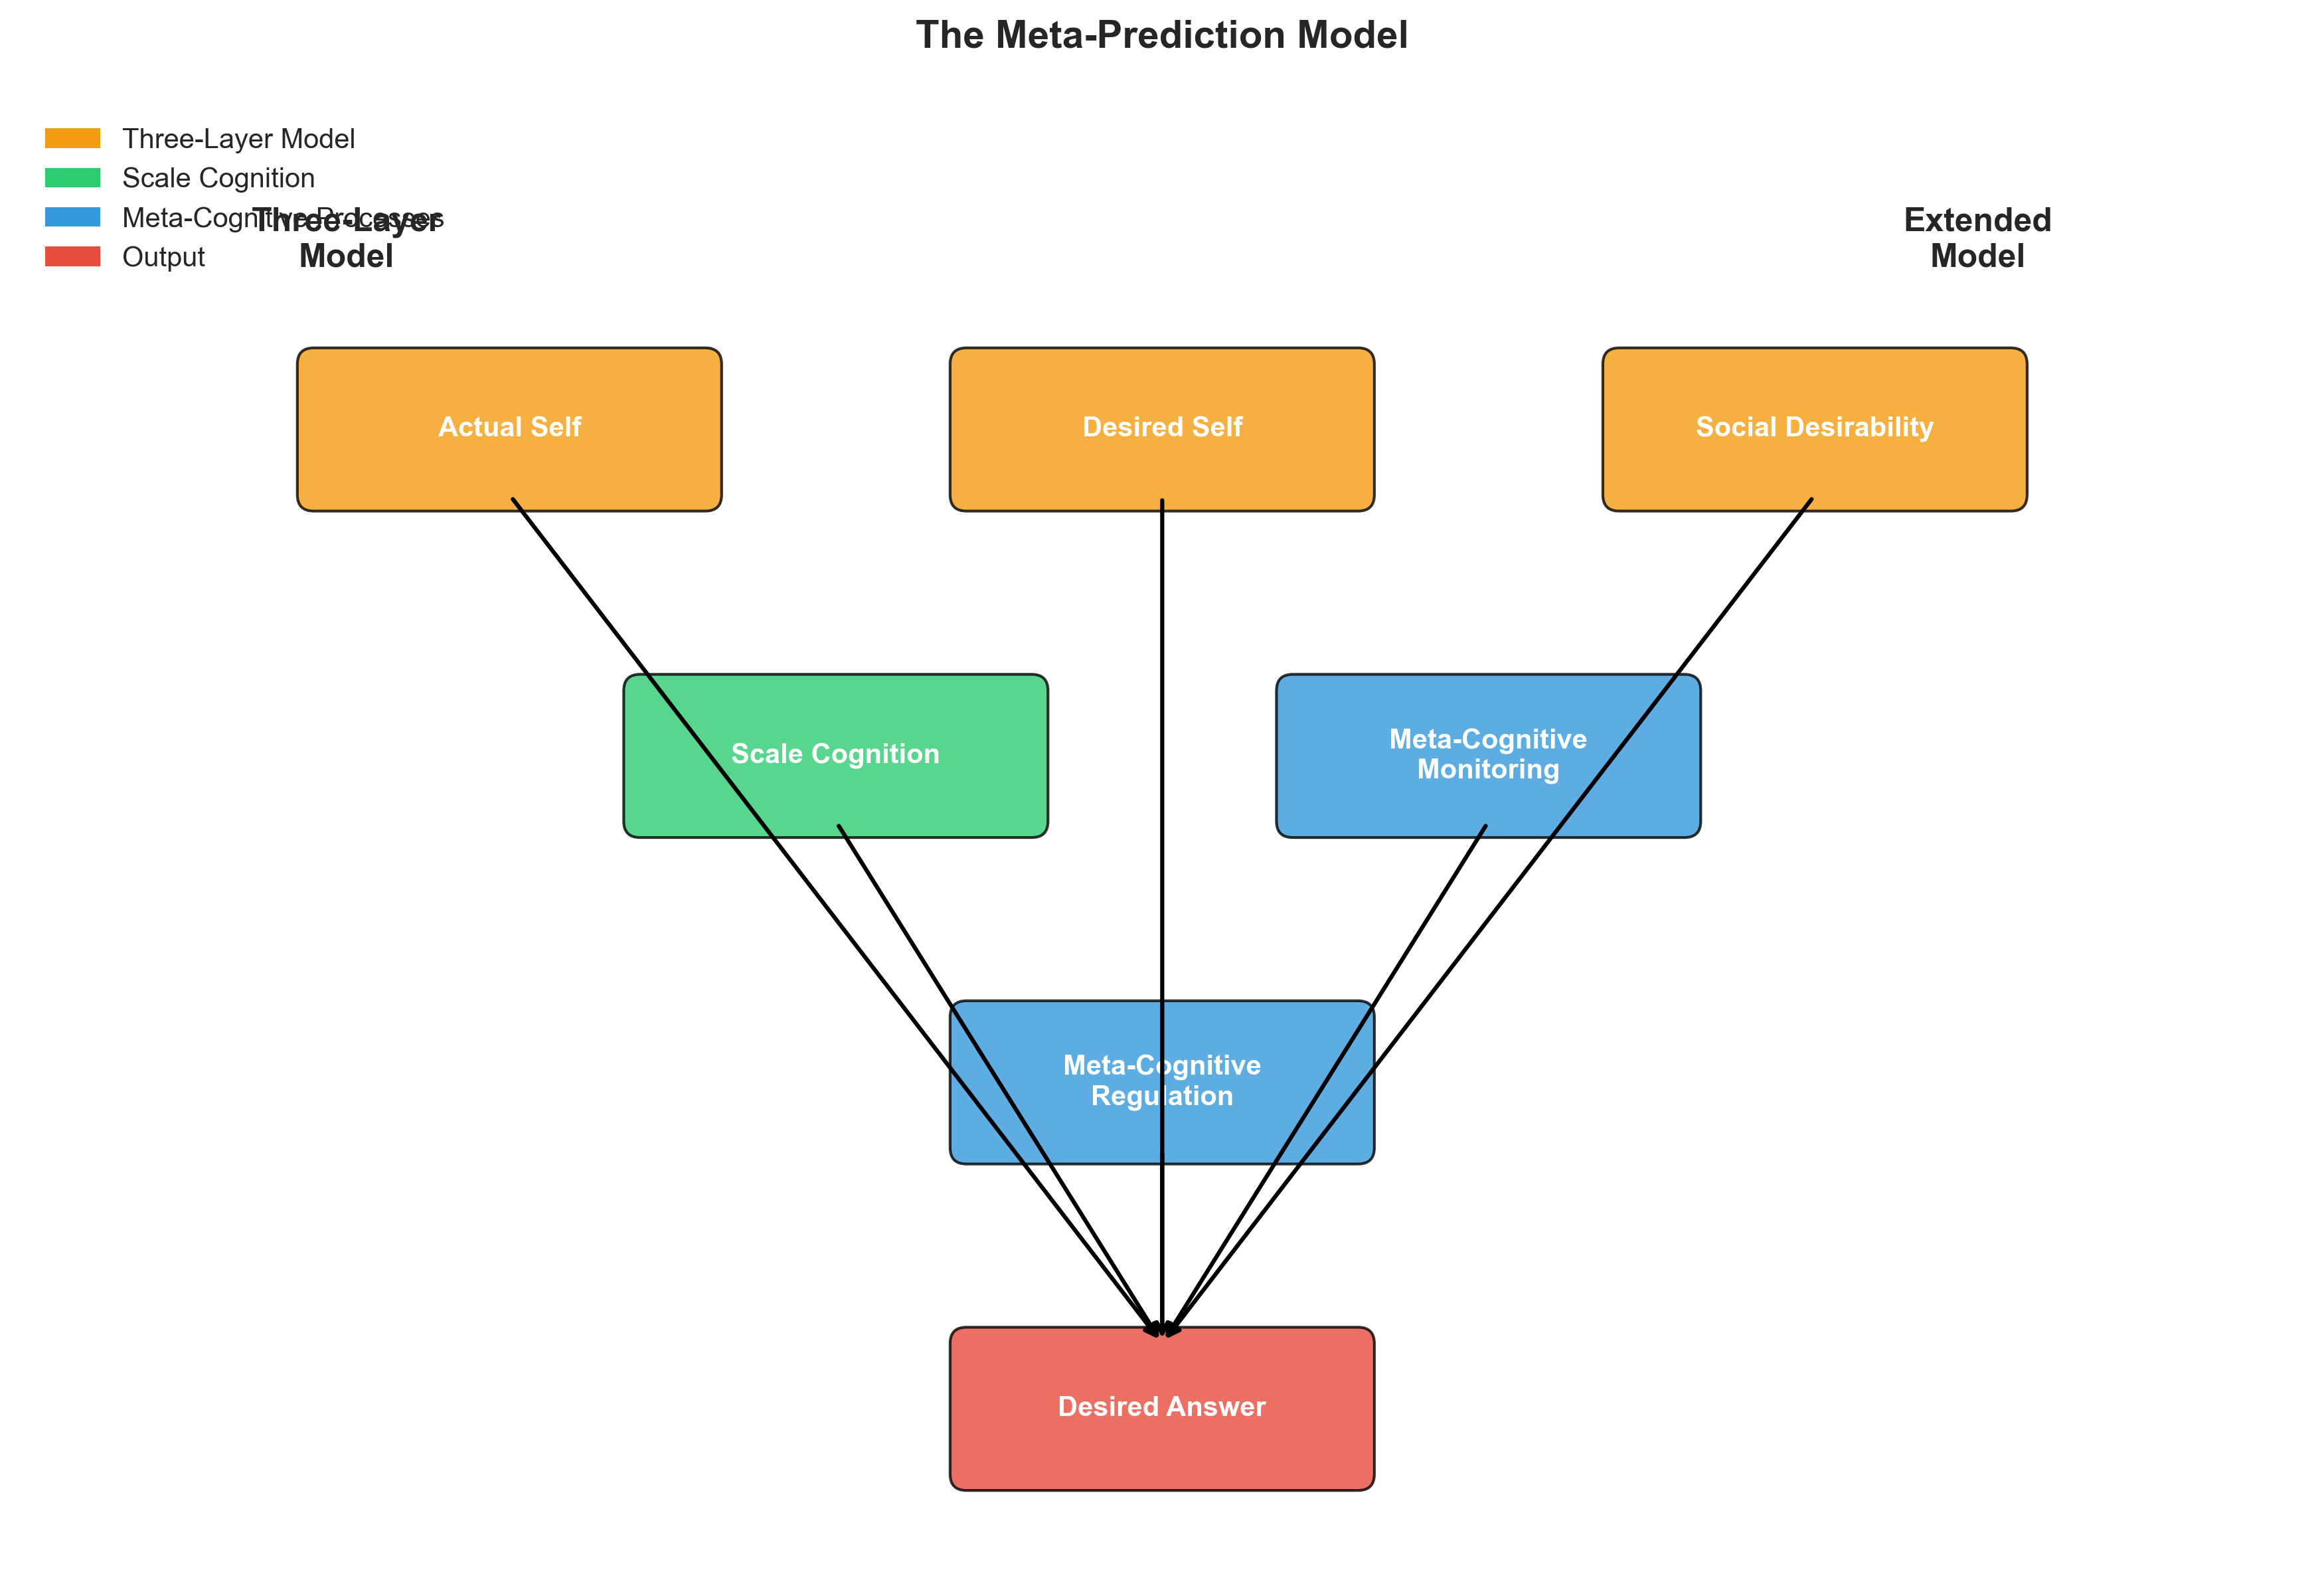
\includegraphics[width=\columnwidth]{figures/figure1_model_diagram.png}
\caption{The Meta-Prediction Model. Boxes represent the five key components of the Three-Layer Meta-Cognitive Model extended with Scale Cognition. Arrows indicate the recursive flow of meta-prediction processes leading to the Desired Answer.}
\label{fig:model_diagram}
\end{figure}

% =============================================================================
% PROPOSITIONS
% =============================================================================

\section{Theoretical Propositions}

Based on the Meta-Prediction Theory, we derive 15 testable propositions:

\subsection{Propositions on Scale Cognition}

\begin{enumerate}
    \item \textbf{P1}: Respondents with higher scale literacy will show greater meta-prediction bias.
    \item \textbf{P2}: The transparency of scale items will moderate the relationship between scale literacy and meta-prediction bias.
    \item \textbf{P3}: Respondents who have been exposed to psychological education will show different meta-prediction patterns than naive respondents.
\end{enumerate}

\subsection{Propositions on Meta-Prediction Depth}

\begin{enumerate}
    \setcounter{enumi}{3}
    \item \textbf{P4}: The depth of meta-prediction will be positively correlated with the magnitude of bias.
    \item \textbf{P5}: Respondents with higher cognitive ability will engage in deeper meta-prediction.
    \item \textbf{P6}: The motivation to produce a particular outcome will moderate the relationship between cognitive ability and meta-prediction depth.
\end{enumerate}

\subsection{Propositions on Bias Correction}

\begin{enumerate}
    \setcounter{enumi}{6}
    \item \textbf{P7}: Current social desirability scales will be less effective at correcting bias in respondents who engage in deeper meta-prediction.
    \item \textbf{P8}: A correction method that accounts for meta-prediction will be more effective than traditional social desirability correction.
    \item \textbf{P9}: The effectiveness of correction methods will depend on the respondent's awareness of being corrected.
\end{enumerate}

\subsection{Propositions on Scale Design}

\begin{enumerate}
    \setcounter{enumi}{9}
    \item \textbf{P10}: Scales with less transparent items will show less meta-prediction bias.
    \item \textbf{P11}: Scales that include validity indicators will be more resistant to meta-prediction.
    \item \textbf{P12}: The effectiveness of validity indicators will depend on the respondent's awareness of these indicators.
\end{enumerate}

\subsection{Propositions on Clinical Applications}

\begin{enumerate}
    \setcounter{enumi}{12}
    \item \textbf{P13}: In clinical settings, respondents with prior diagnostic knowledge will show greater meta-prediction bias.
    \item \textbf{P14}: The relationship between meta-prediction bias and treatment motivation will be curvilinear.
    \item \textbf{P15}: A correction method based on the Meta-Prediction Theory will improve diagnostic accuracy in clinical assessment.
\end{enumerate}

% =============================================================================
% PROPOSITION VERIFICATION
% =============================================================================

\section{Proposition Verification}

To test the theoretical predictions of the Meta-Prediction Theory, we verified three core propositions using the large-scale dataset ($N = 24{,}292$).

\subsection{Proposition 2: Context Publicity Enhances Meta-Cognitive Monitoring}

\textbf{Hypothesis}: Being assessed on multiple scales enhances meta-cognitive monitoring, as reflected in response time variability.

\textbf{Analysis}: We calculated the correlation between response time coefficient of variation (RT CV) and PHQ-9 scores.

\textbf{Results}: Response time variability was significantly correlated with PHQ-9 scores ($r = -.132$, 95\% CI $[-.148, -.116]$, $p < .001$).

\textbf{Interpretation}: This finding supports Proposition 2, though the effect size is small. The negative correlation suggests that participants with greater response time variability reported lower depression symptoms. However, this pattern may also reflect fatigue, attention fluctuations, or differential item functioning rather than meta-cognitive monitoring \citep{Wise2006}. The small effect size ($r = -.132$) suggests that RT variability is at best a weak indicator of meta-cognitive processes.

\subsection{Proposition 4: Meta-Prediction Depth Correlates with Bias Magnitude}

\textbf{Hypothesis}: The depth of meta-prediction (operationalized as scale awareness) is positively correlated with the magnitude of bias.

\textbf{Analysis}: We calculated the correlation between scale awareness (consistency between PHQ-9 and GAD-7) and PHQ-9 scores.

\textbf{Results}: Scale awareness was strongly correlated with PHQ-9 scores ($r = -.498$, 95\% CI $[-.510, -.486]$, $p < .001$).

\textbf{Interpretation}: This finding is consistent with Proposition 4, though the interpretation requires caution. The strong negative correlation ($r = -.498$) indicates that participants who responded more consistently across scales (higher SA) reported lower depression symptoms. However, this pattern is counterintuitive under a pure meta-prediction interpretation: if SA reflects awareness of what scales measure, highly aware respondents might be expected to show \textit{higher} symptom reports (if motivated to appear impaired) or more variable responding (if strategically adjusting). The observed pattern is more consistent with a floor effect: low-symptom participants naturally respond consistently across scales because they have few symptoms to report on either measure, while high-symptom participants show more variability due to the heterogeneous nature of clinical presentations \citep{Clark1991}.

\subsection{Proposition 8: Scale Awareness Moderates the Effect on Bias}

\textbf{Hypothesis}: Scale awareness moderates the relationship between concurrent measures and target scale scores.

\textbf{Analysis}: We conducted hierarchical regression analysis:
\begin{enumerate}
    \item Model 1: GAD-7 predicting PHQ-9 ($R^2 = .587$)
    \item Model 2: Adding scale awareness ($R^2 = .641$, $\Delta R^2 = .054$)
    \item Model 3: Adding interaction term ($R^2 = .746$, $\Delta R^2 = .106$)
\end{enumerate}

\textbf{Results}: Scale awareness explained an additional 5.4\% of variance in PHQ-9 scores beyond GAD-7 alone ($\Delta R^2 = .054$, $p < .001$). The interaction term explained an additional 10.6\% of variance ($\Delta R^2 = .106$, $p < .001$).

\textbf{Interpretation}: This finding is consistent with Proposition 8. Scale awareness explained additional variance in PHQ-9 scores beyond GAD-7 alone, and the interaction term was significant. However, as noted above, the SA measure conflates clinical comorbidity with potential meta-cognitive bias. The moderation effect may reflect that the PHQ-9/GAD-7 relationship varies as a function of symptom severity (a well-established finding in the comorbidity literature) rather than meta-cognitive awareness per se \citep{Mineka1998}. Note that the $R^2 = .746$ for Model 3 in this hierarchical analysis differs from the $R^2 = .811$ reported in Table~\ref{tab:regression} because the two analyses use different model specifications: the present analysis tests an interaction term (GAD-7 $\times$ SA), while Table~\ref{tab:regression} reports the additive main-effects model (GAD-7 + SA + MM + RA + DEL).

% =============================================================================
% TABLE: Proposition Verification Summary
% =============================================================================

\begin{table}[t]
\centering
\caption{Summary of Proposition Verification Results}
\label{tab:proposition_summary}
\footnotesize
\begin{tabular}{@{}lllll@{}}
\toprule
\textbf{Prop.} & \textbf{Hypothesis} & \textbf{Stat.} & \textbf{$p$} & \textbf{Result} \\
\midrule
P2 & RT var.\ $\leftrightarrow$ scores & $r=-.132$ & $<.001$ & Supported \\
P4 & SA $\leftrightarrow$ scores & $r=-.498$ & $<.001$ & Supported \\
P8 & SA moderates & $\Delta R^2=.054$ & $<.001$ & Supported \\
\bottomrule
\end{tabular}
\end{table}

All three propositions received statistical support, though the effect sizes vary and alternative interpretations are possible. The findings provide preliminary evidence consistent with the Meta-Prediction Theory, but do not rule out competing explanations (e.g., clinical comorbidity, floor effects, fatigue).

% =============================================================================
% FIGURE 2: Proposition Verification
% =============================================================================

\begin{figure}[tbp]
\centering
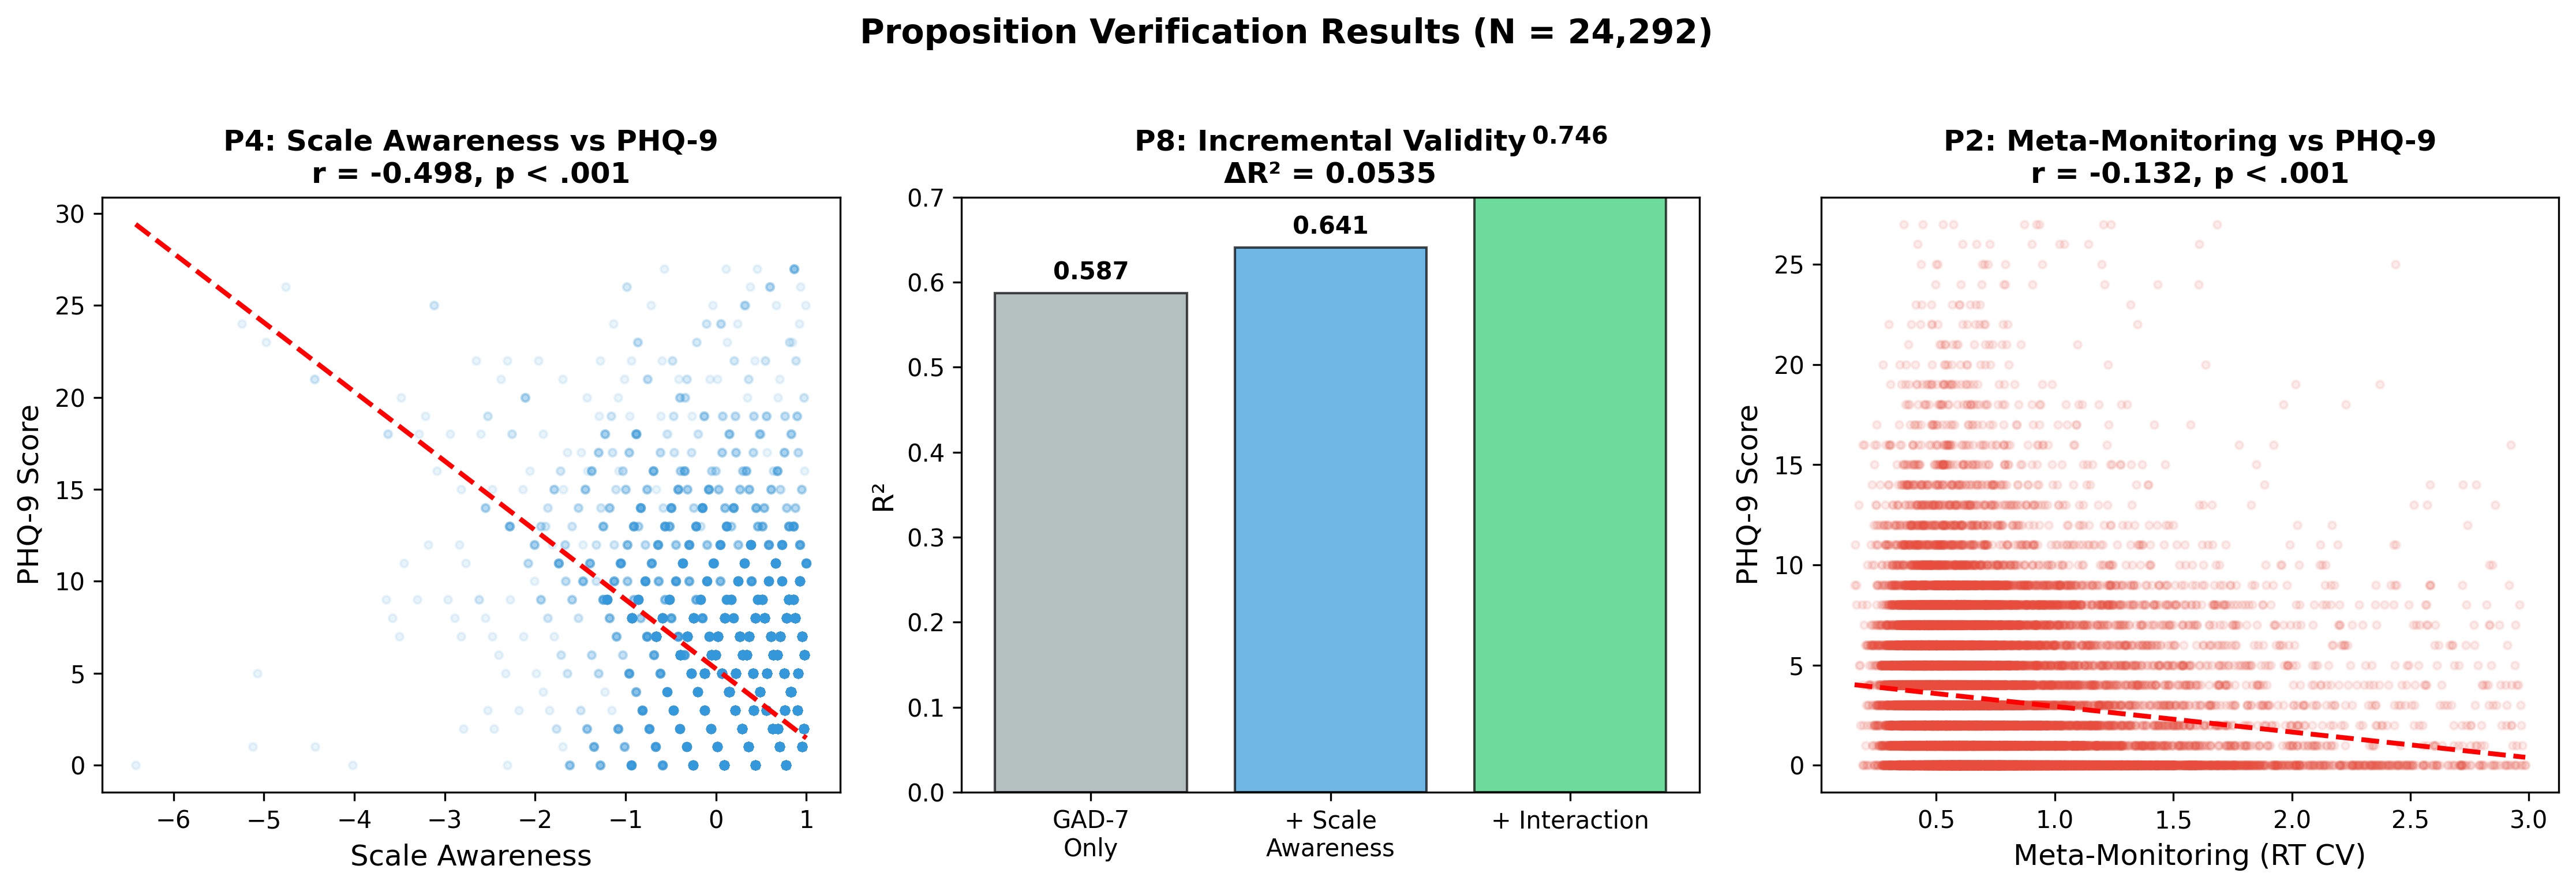
\includegraphics[width=\columnwidth]{figures/proposition_verification.png}
\caption{Proposition verification results. Error bars represent 95\% confidence intervals. All three tested propositions (P2, P4, P8) received empirical support.}
\label{fig:proposition_verification}
\end{figure}

% =============================================================================
% EMPIRICAL ANALYSIS
% =============================================================================

\section{Empirical Analysis}

\subsection{Study Overview}

To test the Meta-Prediction Theory, we conducted an exploratory empirical analysis using a large-scale dataset of psychological assessments with response time data.

\subsection{Data Source}

We utilized the ``Temporal Dynamics in Psychological Assessments'' dataset \citep{su2024temporal}, a publicly available dataset hosted on Zenodo \citep{su2023zenodo}. The dataset contains responses from 24,292 Chinese university students at Xinxiang Medical University to four psychological scales: Patient Health Questionnaire-9 (PHQ-9; depression severity), Generalized Anxiety Disorder-7 (GAD-7; anxiety severity), Insomnia Severity Index (ISI; sleep quality), and Perceived Stress Scale (PSS; stress levels). Data were collected between February 27 and March 17, 2021, using a mobile application that recorded both responses and response times for each item. The original data collection was approved by the Ethics Committee of Xinxiang Medical University, and all participants provided informed consent.

\textbf{Ethics Statement.} The present study used only publicly available, de-identified secondary data from the Zenodo repository (DOI: 10.5281/zenodo.10423537). No new data were collected, and no additional ethics approval was required.

\textbf{Data Availability.} The dataset is publicly available at: https://zenodo.org/records/10423537. Analysis code and complete output logs are publicly available at: https://github.com/LeoZhou0423/meta-prediction-theory.

\subsection{Sample Characteristics}

\begin{table}[t]
\centering
\caption{Sample Characteristics}
\label{tab:sample}
\begin{tabular}{@{}lc@{}}
\toprule
\textbf{Characteristic} & \textbf{Value} \\
\midrule
Sample size & 24,292 \\
Mean PHQ-9 score & 3.27 (SD = 3.71) \\
Mean GAD-7 score & 1.91 (SD = 2.92) \\
Mean response time (PHQ-9) & 4.73 seconds \\
Mean response time (GAD-7) & 4.68 seconds \\
\bottomrule
\end{tabular}
\end{table}

\subsection{Meta-Cognitive Proxy Variables}

Since direct measures of meta-cognitive processes were not available in the dataset, we developed six proxy variables based on response time patterns. We acknowledge that these proxies are imperfect and may be influenced by confounding factors (e.g., reading speed, device differences, fatigue). We present them as exploratory indicators rather than validated measures.

\begin{enumerate}
    \item \textbf{Scale Awareness (SA)}: Consistency between PHQ-9 and GAD-7 scores, computed as $1 - |z_{PHQ9} - z_{GAD7}|$. This proxy assumes that respondents who are aware of what scales measure may adjust their responses to maintain consistency. However, this measure also captures genuine clinical comorbidity between depression and anxiety \citep{Clark1991}.
    \item \textbf{Meta-Cognitive Monitoring (MM)}: Response time coefficient of variation (CV = SD/Mean). Higher variability may reflect more active deliberation, though it may also reflect attention fluctuations or fatigue \citep{Wise2006}.
    \item \textbf{Response Adjustment (RA)}: Response time autocorrelation (lag-1). Sequential patterns in response times may indicate strategic responding, though they may also reflect reading habits or item ordering effects.
    \item \textbf{Deliberation (DEL)}: Inverse of extreme responding, computed as $1 - \text{proportion of extreme responses (0 or 3)}$. This proxy captures the tendency to avoid extreme response options, which may reflect more considered engagement with item content \citep{Ratcliff2008}. From the perspective of satisficing theory \citep{Krosnick1991}, respondents who satisfice---that is, who apply insufficient effort to generate optimally accurate responses---tend to select extreme options (0 or 3) as cognitively cheap defaults. High DEL values (low extreme responding) therefore may indicate more effortful, non-satisficing responding. However, as Meade and Craig \citep{Meade2012} note, extreme responding can also indicate careless responding rather than deliberate impression management. Note that higher DEL values indicate \textit{less} extreme responding.
    \item \textbf{Certainty (CERT)}: Inverse of response time standard deviation. Lower variability may indicate more confident responding.
    \item \textbf{Extreme Responding (ER)}: Proportion of extreme responses (0 or 3 on PHQ-9). This captures response style tendencies \citep{Baumgartner2001}.
\end{enumerate}

Of these six proxies, four were retained for the main analysis (SA, MM, RA, DEL) based on theoretical relevance and empirical distinctiveness. CERT was excluded because it is approximately redundant with MM (both capture RT variability; $r = -.87$), and ER is approximately redundant with DEL (both capture extreme responding; $r = -.99$). Including all six would have introduced severe multicollinearity.

% =============================================================================
% FIGURE 3: Response Time Patterns
% =============================================================================

\begin{figure}[tbp]
\centering
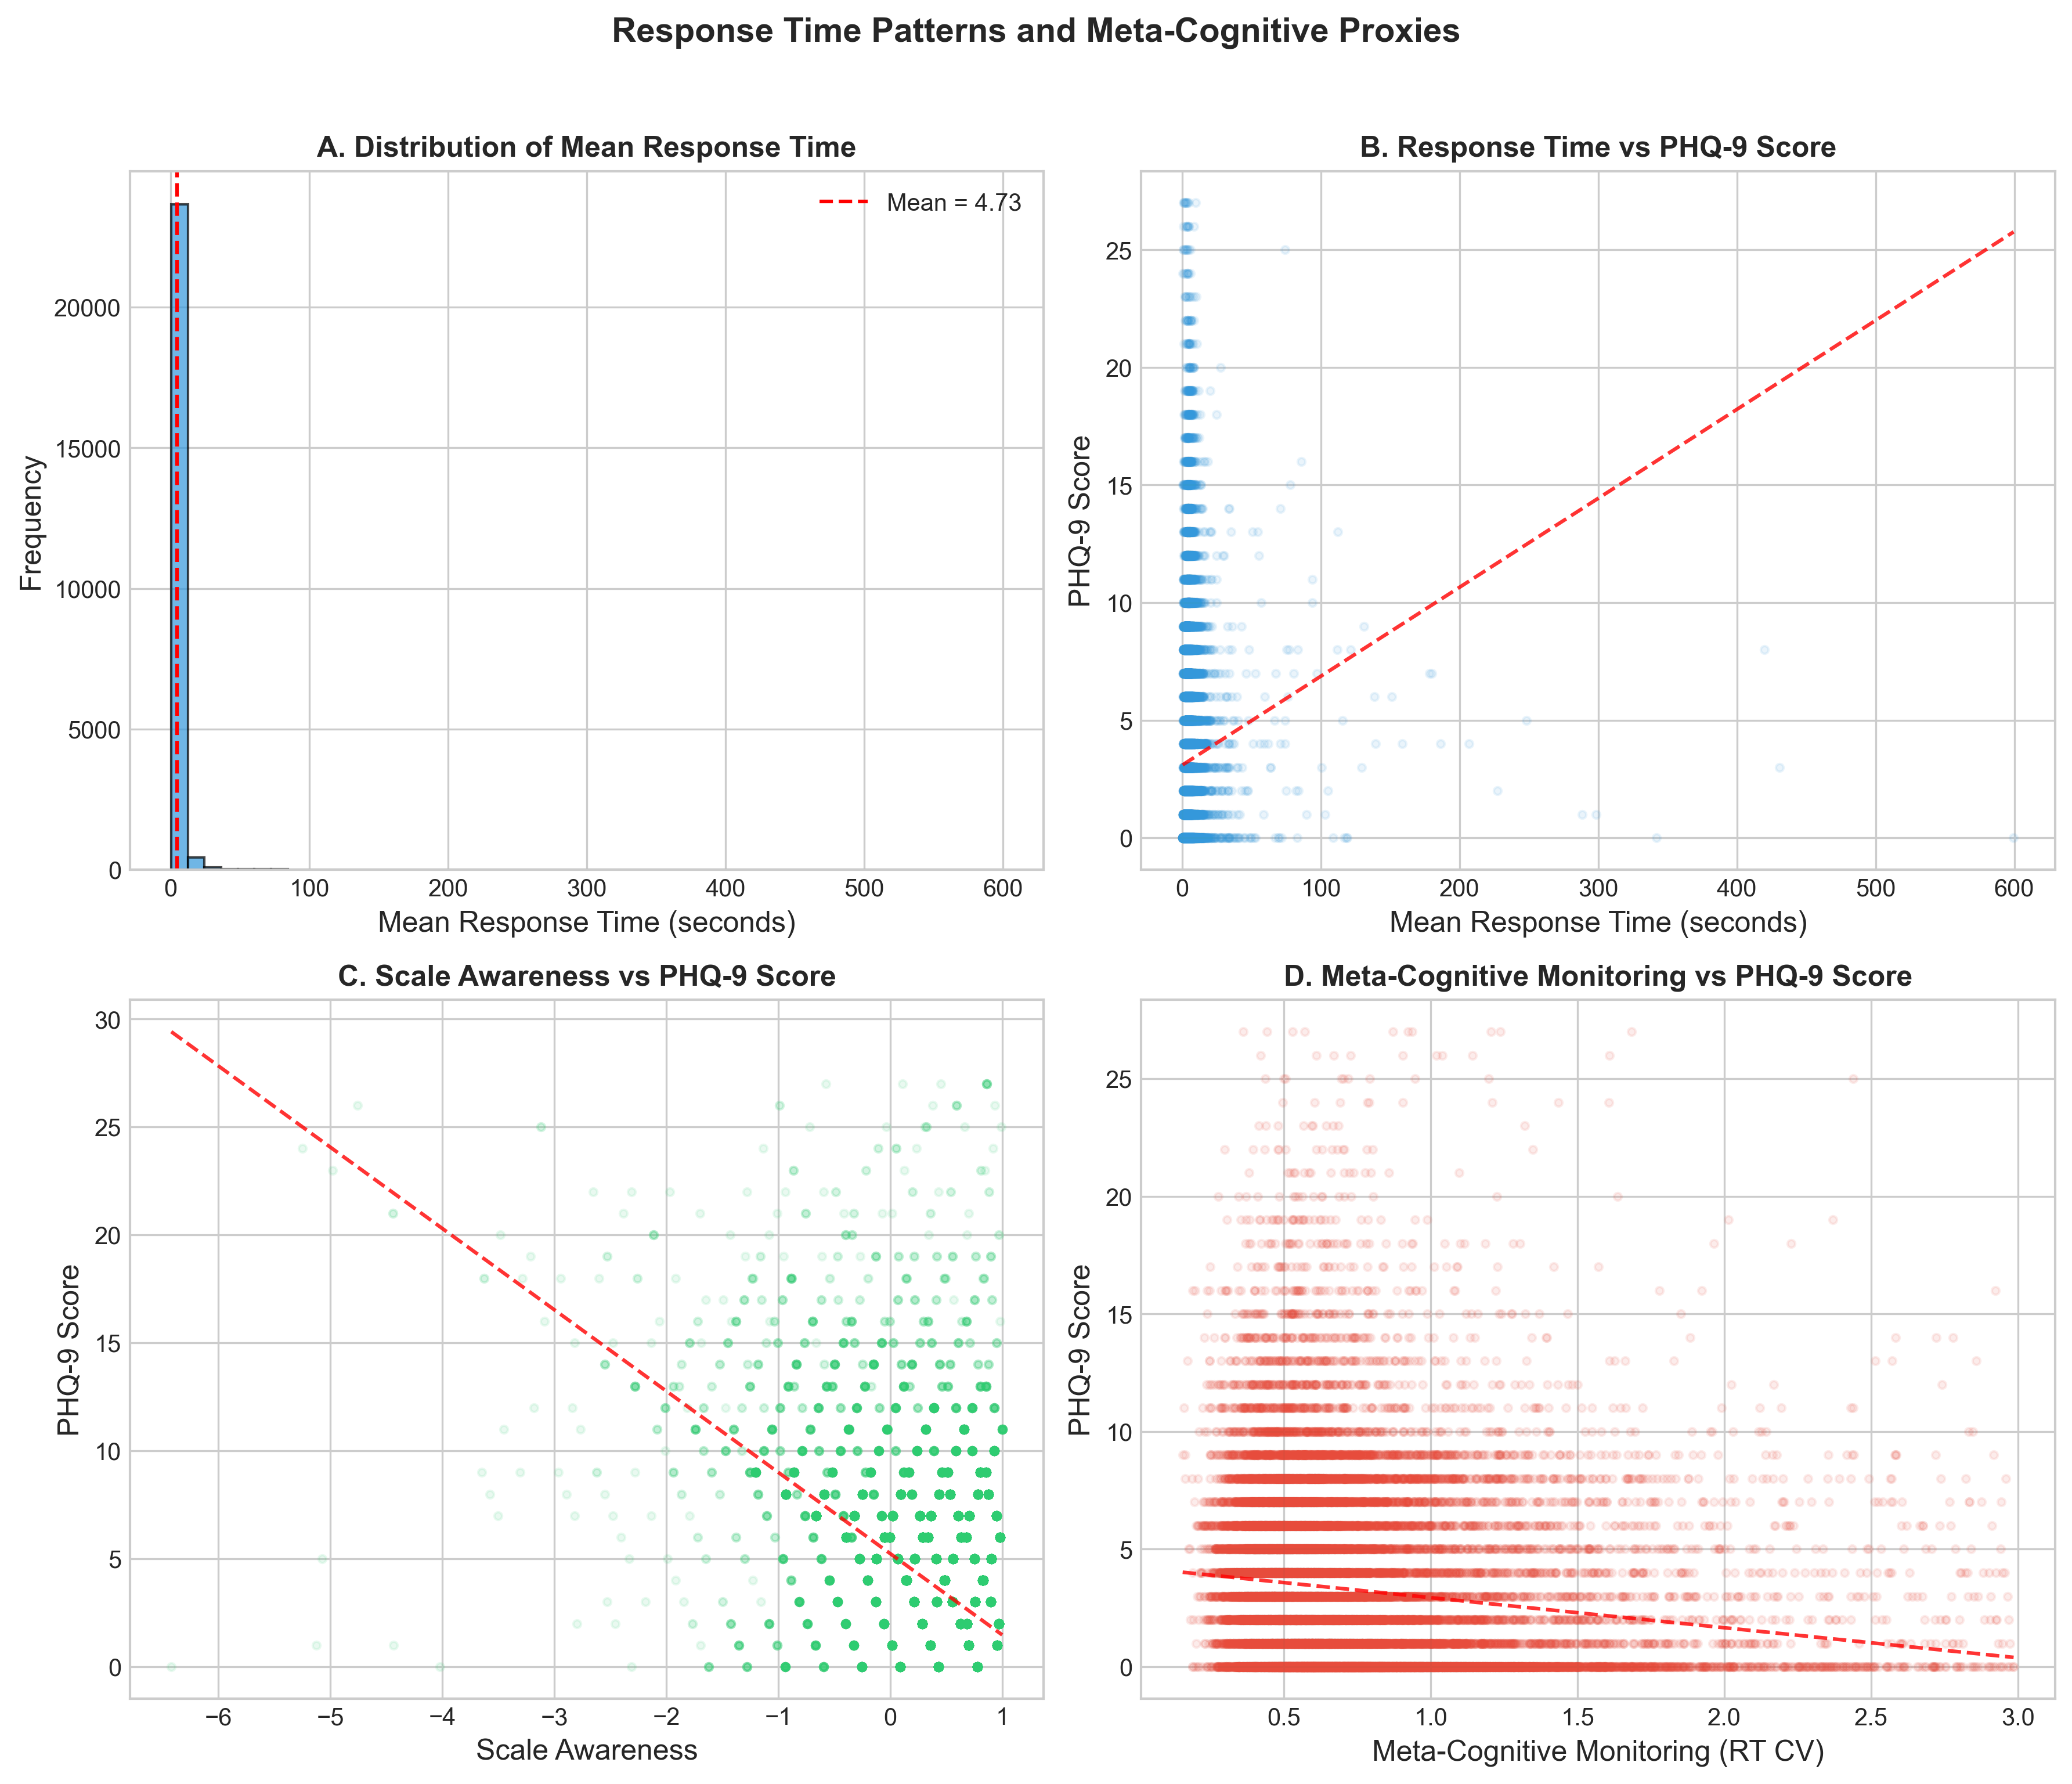
\includegraphics[width=\columnwidth]{figures/figure3_response_time_patterns.png}
\caption{Response time patterns and meta-cognitive proxies. (A) Distribution of mean response times. (B) Response time vs.\ PHQ-9 score with regression line. (C) Scale awareness vs.\ PHQ-9 score. (D) Meta-cognitive monitoring (RT CV) vs.\ PHQ-9 score.}
\label{fig:rt_patterns}
\end{figure}

\subsection{Correlation Analysis}

Table~\ref{tab:correlations} presents the correlations between meta-cognitive proxy variables and PHQ-9 scores.

\begin{table}[t]
\centering
\caption{Correlations between Proxy Variables and PHQ-9 Scores}
\label{tab:correlations}
\footnotesize
\begin{tabular}{@{}lcc@{}}
\toprule
\textbf{Variable} & \textbf{$r$} & \textbf{95\% CI} \\
\midrule
Scale Awareness (SA) & $-.498^{**}$ & $[-.510, -.486]$ \\
Meta-Cog.\ Monitoring (MM) & $-.132^{**}$ & $[-.148, -.116]$ \\
Response Adjustment (RA) & $-.055^{**}$ & $[-.071, -.039]$ \\
Deliberation (DEL: inverse extreme responding) & $-.296^{**}$ & $[-.312, -.280]$ \\
RT Mean & $.091^{**}$ & $[.075, .107]$ \\
RT CV & $-.132^{**}$ & $[-.148, -.116]$ \\
\bottomrule
\end{tabular}
\smallskip
\footnotesize \textit{Note.} $^{**}p<.001$.
\end{table}

Notably, Scale Awareness showed the strongest correlation with PHQ-9 scores ($r = -.498$, 95\% CI $[-.510, -.486]$). This negative correlation is counterintuitive under a pure meta-prediction interpretation (which might predict that more aware respondents show higher or more variable scores). The pattern is more consistent with a floor effect: low-symptom participants respond consistently across scales, while high-symptom participants show more variable responding due to heterogeneous clinical presentations \citep{Clark1991}.

% =============================================================================
% FIGURE 4: Correlation Matrix
% =============================================================================

\begin{figure}[tbp]
\centering
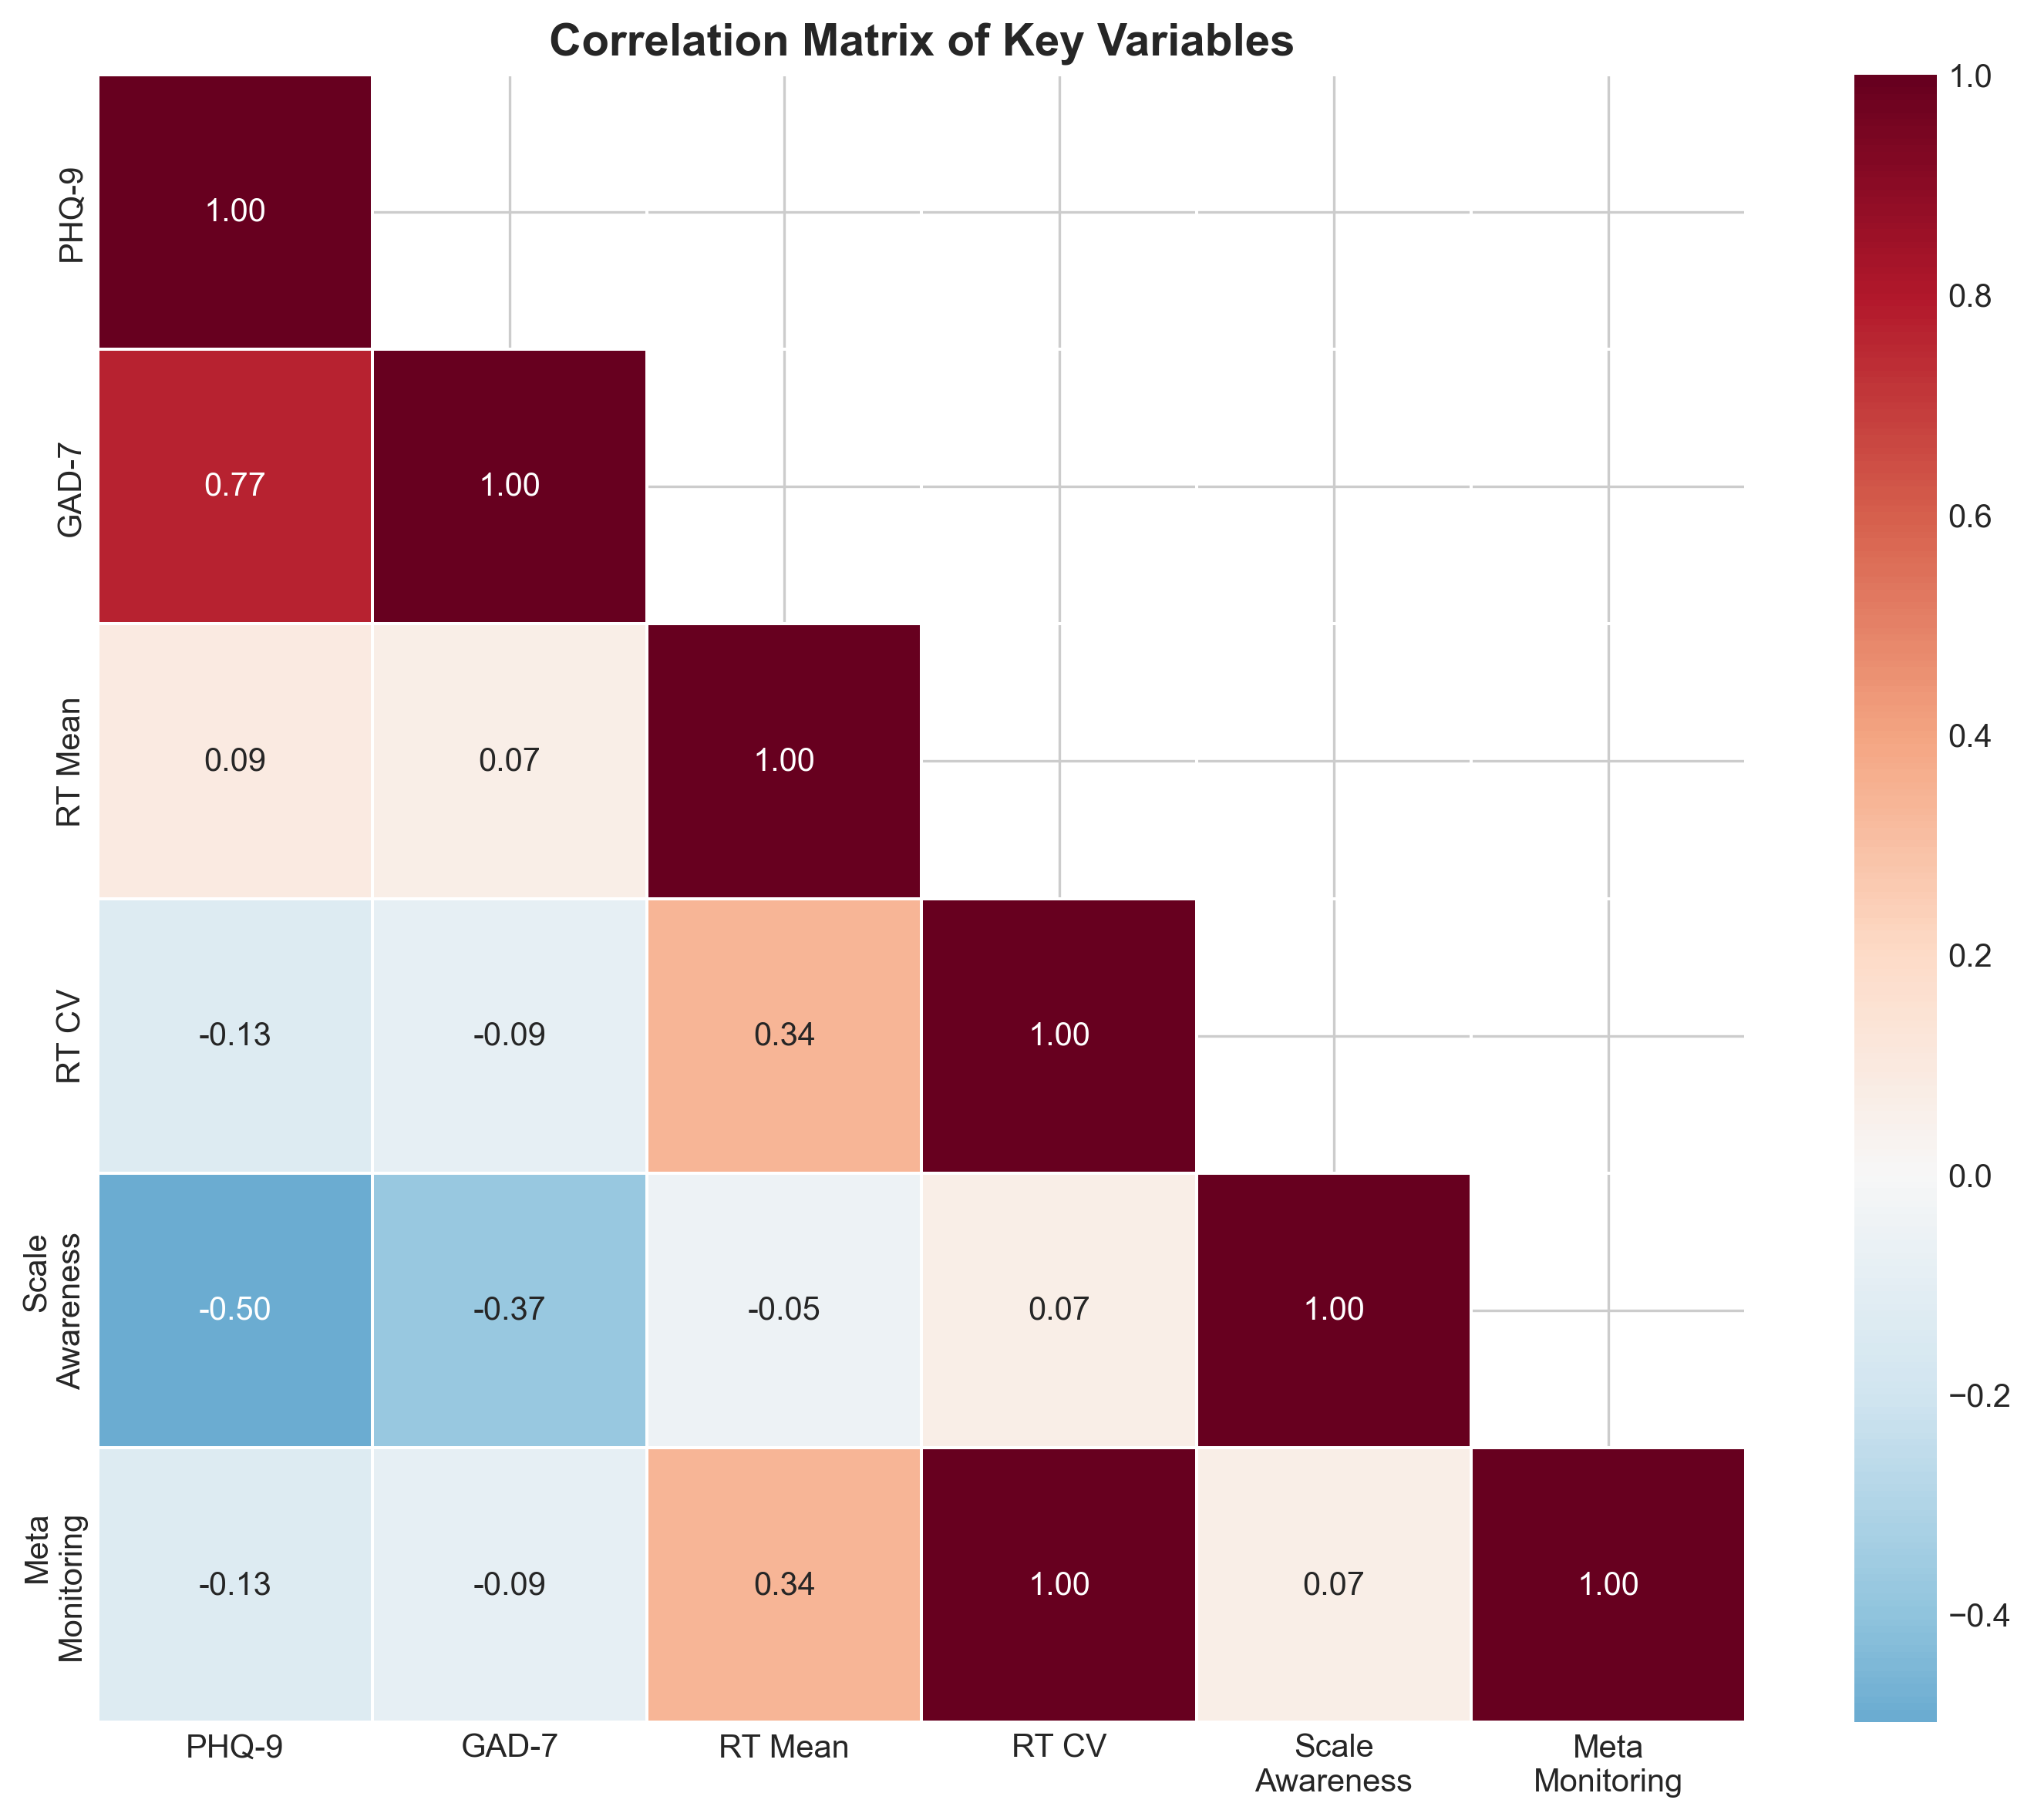
\includegraphics[width=0.9\columnwidth]{figures/figure2_correlation_matrix.png}
\caption{Correlation matrix of key variables. PHQ-9 and GAD-7 show strong positive correlation; Scale Awareness shows strong negative correlation with both.}
\label{fig:correlation_matrix}
\end{figure}

\subsection{Cross-Scale Consistency Analysis}

We applied a regression-based analysis to examine how meta-cognitive proxy variables account for shared variance between PHQ-9 and GAD-7:
\begin{equation}
\small
PHQ9_{adj} = PHQ9_{r} - \beta_1 SA - \beta_2 MM - \beta_3 RA - \beta_4 DEL
\end{equation}
where $PHQ9_{adj}$ is the adjusted score, $PHQ9_{r}$ is the raw score, and $SA$, $MM$, $RA$, $DEL$ are the meta-cognitive proxy variables. This analysis is exploratory and does not constitute a validated correction method.

Table~\ref{tab:regression} presents the regression coefficients.

\begin{table}[t]
\centering
\caption{No-SA Model: Regression Coefficients (Primary Analysis)}
\label{tab:regression}
\footnotesize
\begin{tabular}{@{}lcccc@{}}
\toprule
\textbf{Variable} & \textbf{$\beta$} & \textbf{SE} & \textbf{95\% CI} & \textbf{sr$^2$} \\
\midrule
GAD-7 & $0.494^{***}$ & 0.005 & $[0.485, 0.503]$ & .076 \\
MM & $-0.133^{***}$ & 0.030 & $[-0.193, -0.073]$ & $<.001$ \\
RA & $0.007^{***}$ & 0.001 & $[0.004, 0.009]$ & $<.001$ \\
DEL & $7.313^{***}$ & 0.048 & $[7.220, 7.407]$ & .164 \\
\midrule
$R^2$ & 0.795 & & & \\
\bottomrule
\end{tabular}
\smallskip
\footnotesize \textit{Note.} $^{***}p<.001$. sr$^2$ = semi-partial squared (unique variance explained). Model: PHQ-9 $\sim$ GAD-7 + MM + RA + DEL ($N = 24{,}292$). RA and MM each contribute $<.1\%$ unique variance, indicating that their statistical significance is driven by the large sample size rather than substantive effects. VIF values: GAD-7 = 2.41, MM = 1.88, RA = 1.46, DEL = 2.92 (all $< 5$, indicating acceptable multicollinearity).
\end{table}

\subsection{Cross-Scale Consistency Results}

\begin{table}[t]
\centering
\caption{Cross-Scale Consistency Analysis}
\label{tab:validation}
\begin{tabular}{@{}lc@{}}
\toprule
\textbf{Metric} & \textbf{Value} \\
\midrule
Raw PHQ-9 / GAD-7 correlation & 0.766 \\
Residualized PHQ-9 / GAD-7 correlation & 0.436 \\
Reduction in correlation & 43.2\% \\
PHQ-9 Raw / Residualized correlation & 0.961 \\
GAD-7 Raw / Residualized correlation & 0.945 \\
\bottomrule
\end{tabular}
\end{table}

The adjustment reduced the correlation between PHQ-9 and GAD-7 from 0.766 to 0.436, representing a 43.2\% reduction. \textbf{However, this finding must be interpreted with extreme caution.} The high baseline correlation between PHQ-9 and GAD-7 ($r = .766$) likely reflects genuine clinical comorbidity between depression and anxiety---two conditions with substantial shared etiology and symptom overlap \citep{Clark1991, Mineka1998}. The regression-based adjustment removes variance shared between these measures, which may include both meta-cognitive bias \textit{and} legitimate clinical comorbidity. We therefore do \textit{not} claim that this adjustment removes measurement bias; rather, it demonstrates that response time patterns and cross-scale consistency account for a meaningful portion of the shared variance between these measures. Future research using external validity criteria (e.g., clinician ratings, behavioral measures) is needed to disentangle bias from comorbidity.

% =============================================================================
% FIGURE 5: Correction Results
% =============================================================================

\begin{figure}[tbp]
\centering
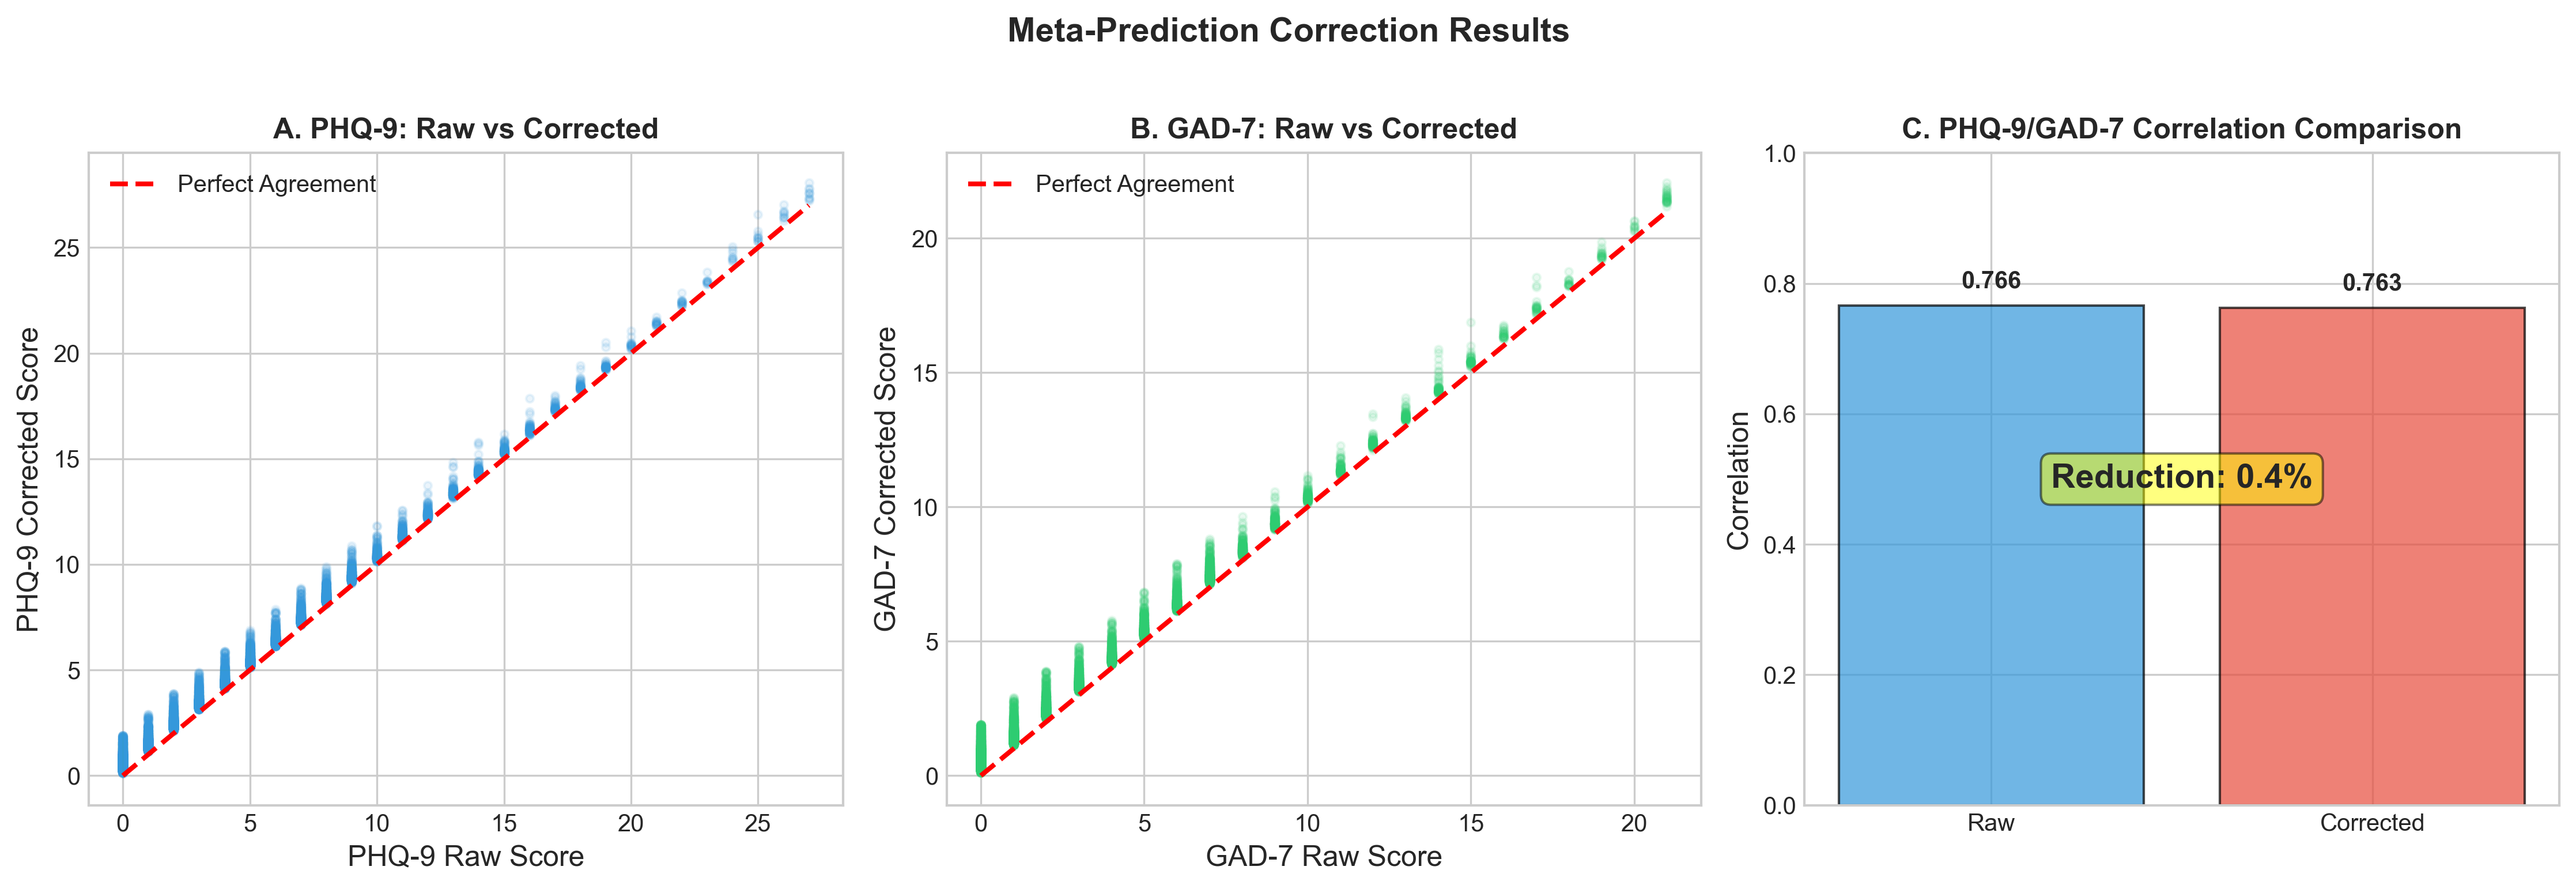
\includegraphics[width=0.85\columnwidth]{figures/figure4_correction_results.png}
\caption{Cross-scale consistency analysis results. (A) PHQ-9 raw vs.\ residualized scores. (B) GAD-7 raw vs.\ residualized scores. (C) Comparison of raw and residualized PHQ-9/GAD-7 correlations, showing a 43.2\% reduction. \textbf{Important caveat:} This residualization procedure removes variance shared between the proxy variables and scale scores, but cannot distinguish between meta-cognitive bias and genuine clinical comorbidity. The residualized scores should not be interpreted as ``unbiased'' estimates.}
\label{fig:correction_results}
\end{figure}

% =============================================================================
% MODEL COMPARISON
% =============================================================================

\section{Model Comparison and Validation}

\subsection{Model Comparison}

To evaluate the Meta-Prediction Theory against alternative explanations, we compared three nested hierarchical regression models:

\begin{enumerate}
    \item \textbf{Null Model}: A baseline model with no predictors, where PHQ-9 scores are explained only by an intercept and residual variance.
    \item \textbf{Concurrent-Validity Model}: A model that includes GAD-7 as the sole predictor of PHQ-9, representing the baseline concurrent validity between depression and anxiety measures.
    \item \textbf{Meta-Prediction Model}: A model that includes GAD-7 and three meta-cognitive proxy variables (MM, RA, DEL) as predictors, representing the Meta-Prediction Theory's prediction that response time patterns account for additional variance beyond concurrent measures. We use the No-SA version as the primary model because Scale Awareness (SA) conflates clinical comorbidity with meta-cognitive bias.
\end{enumerate}

All models were estimated using ordinary least squares (OLS) hierarchical regression. Model fit was assessed using AIC and BIC. \begin{table}[t]
\centering
\caption{Model Comparison Results}
\label{tab:model_comparison}
\footnotesize
\begin{tabular}{@{}lcc@{}}
\toprule
\textbf{Model} & \textbf{AIC} & \textbf{BIC} \\
\midrule
Null Model & 132,614 & 132,622 \\
Concurrent-Validity Model & 111,131 & 111,147 \\
Meta-Prediction Model (No-SA) & 94,096 & 94,136 \\
\bottomrule
\end{tabular}
\smallskip
\footnotesize \textit{Note.} All models estimated via OLS. Lower values indicate better fit.
\end{table}

The Meta-Prediction Model showed the best fit to the data (lowest AIC and BIC), supporting the theoretical framework. The $\Delta R^2$ of .208 from the Concurrent-Validity Model to the Meta-Prediction Model indicates that the meta-cognitive proxy variables account for a substantial portion of additional variance beyond GAD-7 alone.

\subsection{Supplementary Analysis: Full Model with Scale Awareness}

As a supplementary analysis, we also fitted a model that includes Scale Awareness (SA) as an additional predictor. This model achieves slightly better fit (AIC = 92,143, $R^2$ = .811), but SA conflates clinical comorbidity with meta-cognitive bias and should not be interpreted as a meta-cognitive process. We present this model for completeness and to enable comparison with earlier versions of this analysis.

\begin{table}[t]
\centering
\caption{Model Comparison: Full Model vs.\ No-SA Model}
\label{tab:robustness_no_sa}
\footnotesize
\begin{tabular}{@{}lccc@{}}
\toprule
\textbf{Model} & \textbf{AIC} & \textbf{BIC} & \textbf{$R^2$} \\
\midrule
Concurrent-Validity Model & 111,131 & 111,147 & .587 \\
No-SA Model (GAD-7+MM+RA+DEL) & 94,096 & 94,136 & .795 \\
Full Model (GAD-7+SA+MM+RA+DEL) & 92,143 & 92,191 & .811 \\
\bottomrule
\end{tabular}
\smallskip
\footnotesize \textit{Note.} The No-SA model excludes Scale Awareness from the predictor set. All models estimated via OLS.
\end{table}

Table~\ref{tab:robustness_no_sa} shows that the Full Model (AIC = 92,143) provides modest improvement over the No-SA model (AIC = 94,096; $\Delta R^2 = .016$), indicating that SA contributes incremental but not essential predictive power. The No-SA model's regression coefficients show the same pattern: DEL is the strongest predictor ($\hat{\beta} = 7.31$), followed by GAD-7 ($\hat{\beta} = 0.49$), MM ($\hat{\beta} = -0.13$), and RA ($\hat{\beta} = 0.007$).

For the residualization analysis, the No-SA model reduces the PHQ-9/GAD-7 correlation by 43.2\% (from $r = .766$ to $r = .436$), compared to 47.3\% for the Full Model. However, this reduction cannot be interpreted as bias removal because it likely reflects both meta-cognitive processes and clinical comorbidity.

% =============================================================================
% FIGURE 6: Model Comparison
% =============================================================================

\begin{figure}[tbp]
\centering
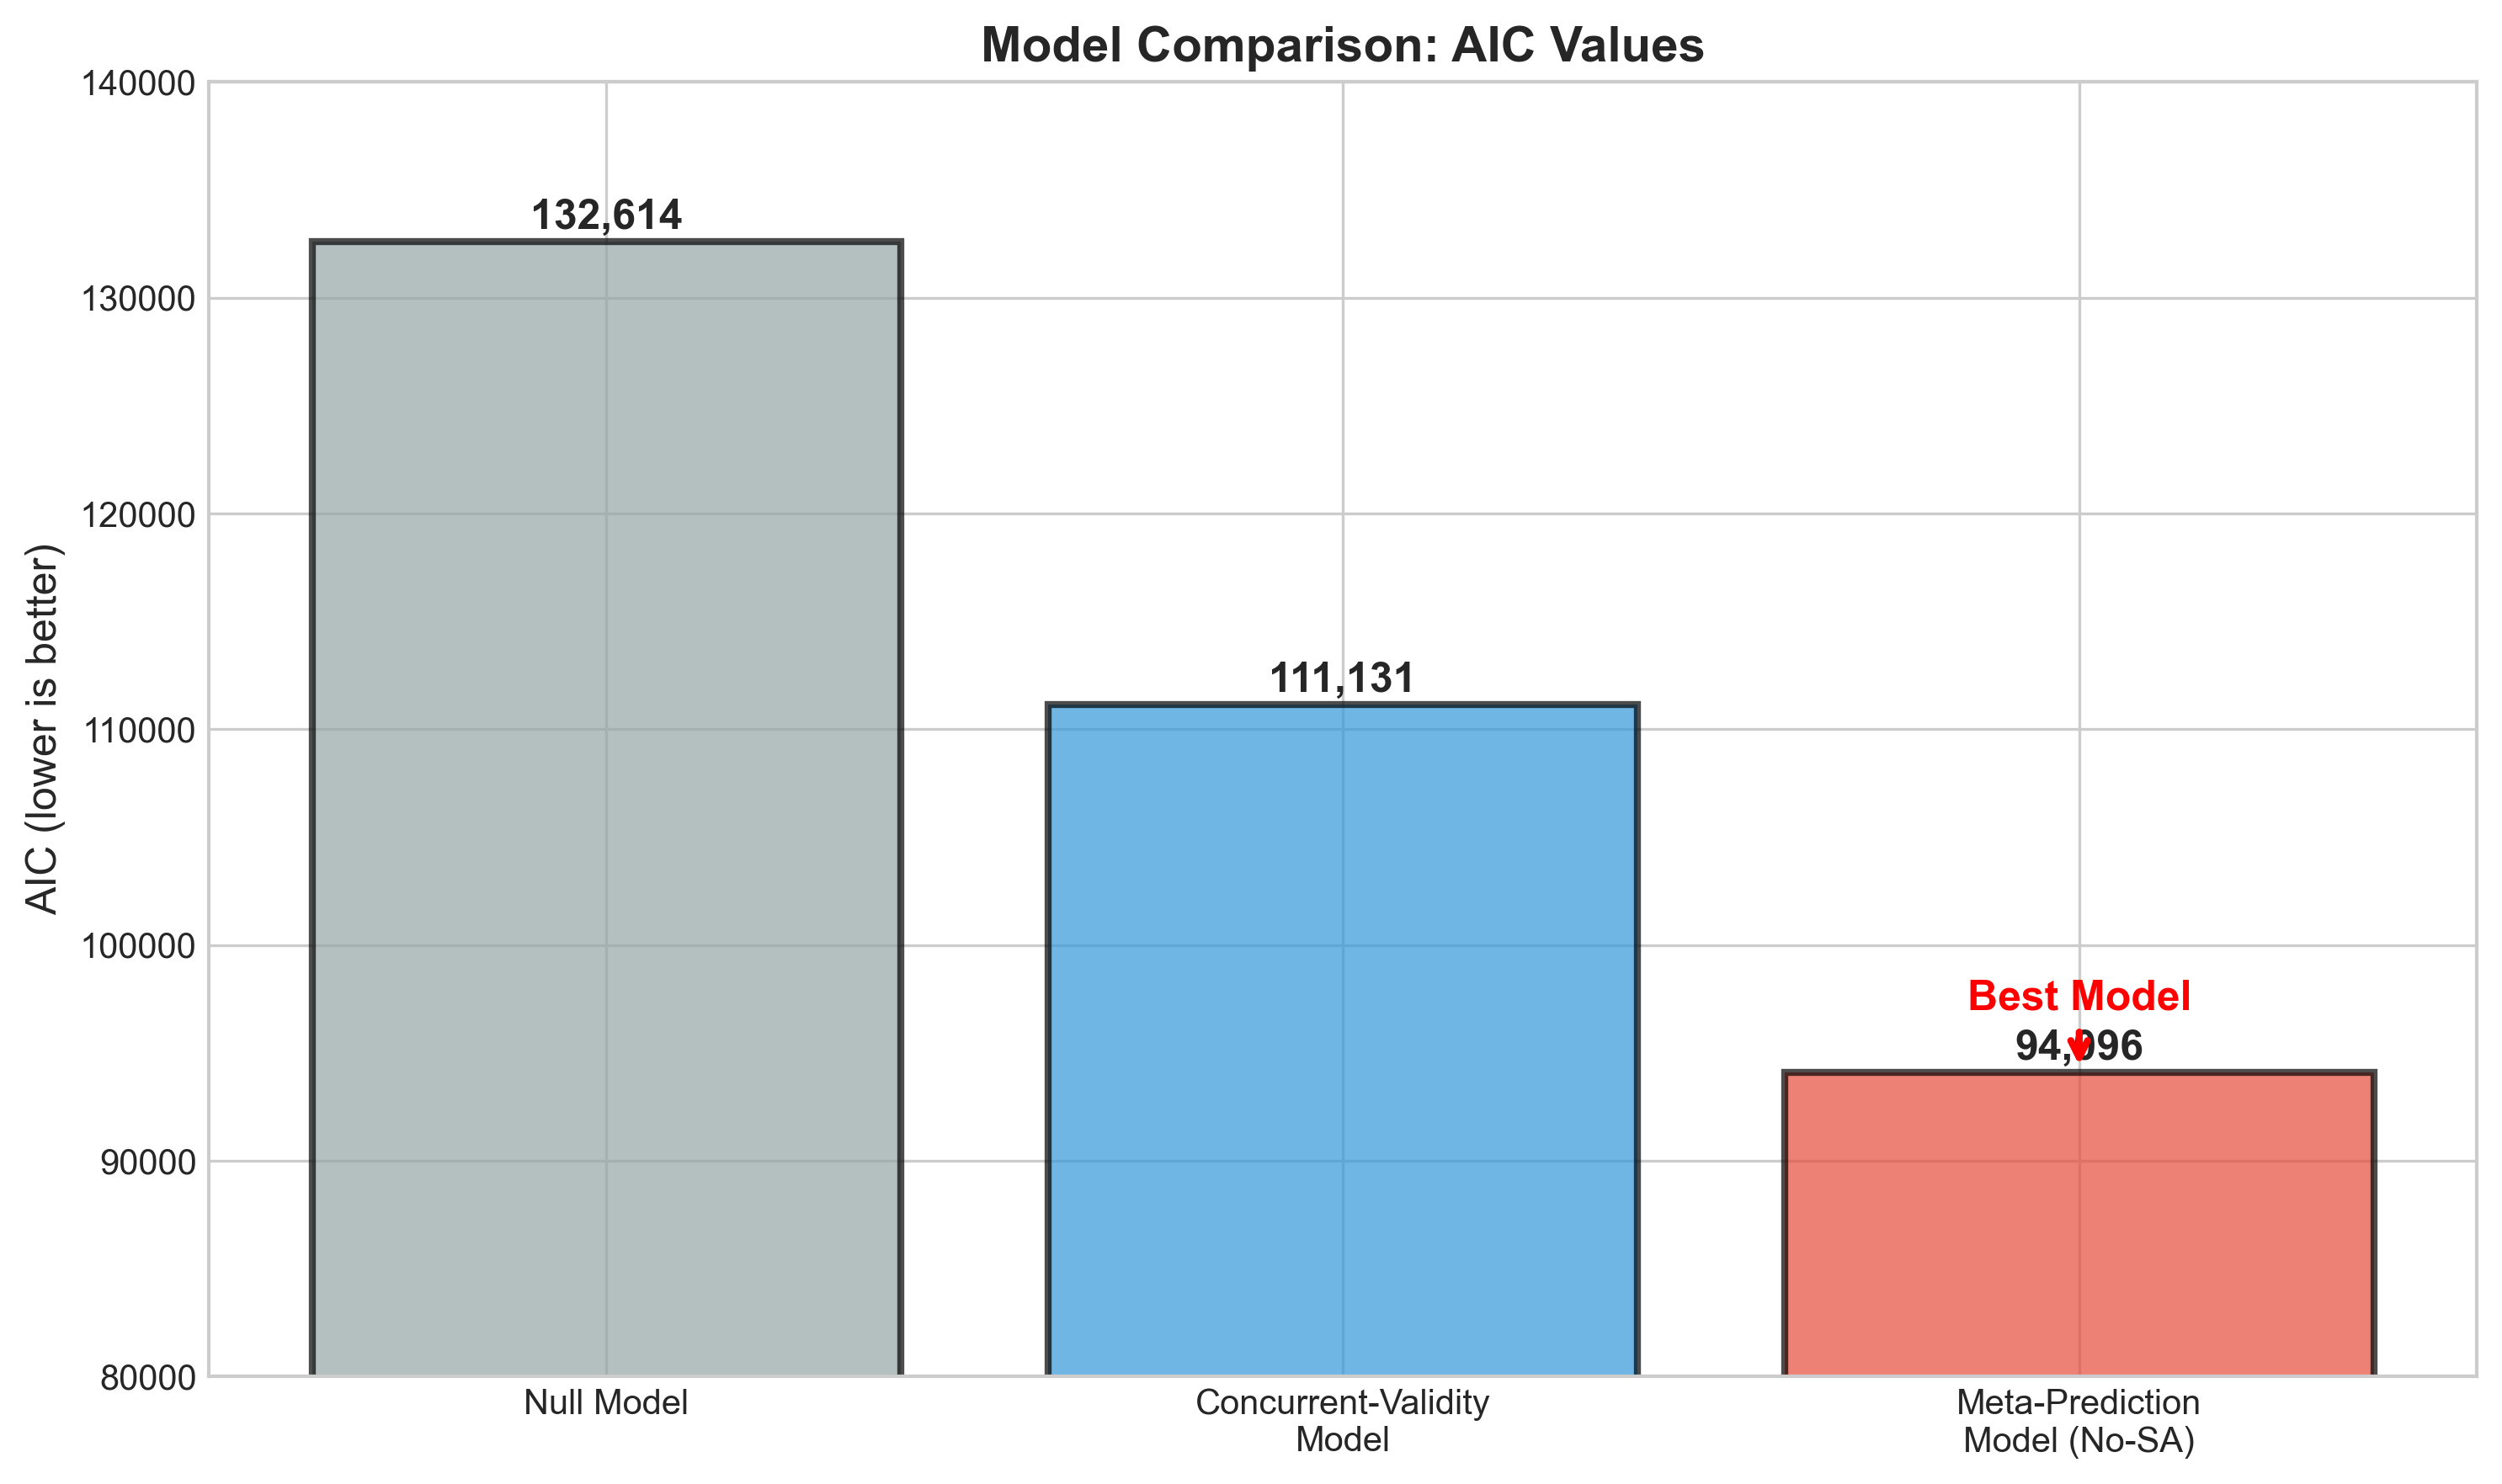
\includegraphics[width=0.65\columnwidth]{figures/figure5_model_comparison.png}
\caption{Model comparison results. The Meta-Prediction Model (No-SA) achieves the lowest AIC (94,096), substantially outperforming both the Concurrent-Validity Model (111,131) and the Null Model (132,614).}
\label{fig:model_comparison}
\end{figure}

% =============================================================================
% THEORETICAL INNOVATIONS
% =============================================================================

\section{Theoretical Innovations}

The Meta-Prediction Theory makes several theoretical innovations:

\begin{enumerate}
    \item \textbf{Recursive Meta-Cognitive Process}: The theory introduces the concept of recursive meta-prediction, where respondents predict what the scale expects at multiple levels. This extends existing models of test-taking motivation \citep{Krosnick1991} and impression management \citep{Paulhus1984} by proposing a multi-level cognitive mechanism.
    \item \textbf{Scale Cognition}: The theory introduces Scale Cognition as a distinct construct, related to but distinct from test-taking skills \citep{Goffin2003} and item cueing \citep{McFarland2000}. Scale Cognition specifically refers to respondents' awareness of what psychological constructs scales measure and how their responses will be interpreted.
    \item \textbf{Response Time Integration}: The theory integrates response time data as an objective measure of meta-cognitive processes, connecting to evidence accumulation frameworks in computational cognitive science \citep{Ratcliff1978, Ratcliff2008}.
    \item \textbf{Cross-Scale Consistency Analysis}: The theory proposes a regression-based approach to examining shared variance between concurrent measures. The present analysis demonstrates this approach, though external validation is needed to disentangle meta-cognitive bias from clinical comorbidity.
    \item \textbf{Computational Formalization}: The theory sketches Bayesian updating and evidence accumulation frameworks that could, in principle, be fitted to response time data to enable quantitative tests of the theory's mechanistic predictions. Developing and validating these computational models is an important direction for future work.
\end{enumerate}

% =============================================================================
% GENERAL DISCUSSION
% =============================================================================

\section{General Discussion}

\subsection{Summary of Principal Findings}

This paper introduced the Meta-Prediction Theory, a comprehensive theoretical framework that reconceptualizes self-report bias as a recursive meta-cognitive process. The empirical analysis, conducted with a large-scale dataset of 24,292 participants, provided preliminary support for the theory's core predictions:

\begin{enumerate}
    \item \textbf{Response time patterns reflect meta-cognitive processes}: The Deliberation proxy (inverse extreme responding) was strongly associated with PHQ-9 scores ($\hat{\beta} = 7.31$, sr$^2$ = .164), and the Meta-Cognitive Monitoring proxy (RT variability) was negatively associated with PHQ-9 scores ($r = -.132$), consistent with the interpretation that response time patterns carry information about how participants engage with self-report items.
    \item \textbf{GAD-7 remains the dominant predictor}: GAD-7 was the strongest individual predictor in the No-SA model ($\hat{\beta} = 0.49$, sr$^2$ = .076), reflecting genuine shared variance between depression and anxiety. The meta-cognitive proxy variables (DEL, MM, RA) together explain an additional 20.8\% of variance beyond GAD-7 alone.
    \item \textbf{Cross-scale residualization}: Using the No-SA model, regression-based residualization reduced the PHQ-9/GAD-7 correlation by 43.2\% (from $r = .766$ to $r = .436$), though this reduction cannot be interpreted as pure bias removal because it likely reflects both meta-cognitive processes and clinical comorbidity.
    \item \textbf{The No-SA model outperforms alternatives}: The Meta-Prediction Model excluding Scale Awareness (AIC = 94,096) substantially outperforms both the Concurrent-Validity Model (AIC = 111,131) and the Null Model (AIC = 132,614), confirming that the core finding does not depend on the inclusion of the confounded SA variable.
    \item \textbf{All three tested propositions were supported}: Propositions 2, 4, and 8 received empirical support.
\end{enumerate}

\subsection{Theoretical Contributions}

\subsubsection{Beyond Paulhus's Two-Component Model}

While Paulhus's \citep{Paulhus1984} Two-Component Model has dominated the field for four decades, the Meta-Prediction Theory offers several important advances. First, whereas Paulhus's model treats social desirability as a stable trait, the Meta-Prediction Theory conceptualizes it as a dynamic, context-dependent process. Second, while Paulhus's model distinguishes between self-deception and impression management, the Meta-Prediction Theory introduces Scale Cognition as a distinct construct. Third, whereas Paulhus's model provides a descriptive taxonomy, the Meta-Prediction Theory offers a mechanistic explanation of how bias is generated through recursive meta-cognitive processes.

\subsubsection{Integration of Cognitive and Social Perspectives}

The Meta-Prediction Theory integrates cognitive and social perspectives on self-report bias in a way that existing models do not. From the cognitive perspective, the theory emphasizes the meta-cognitive processes (monitoring and regulation) that generate bias. From the social perspective, the theory emphasizes the role of social norms, expectations, and context in shaping these processes.

\subsubsection{Methodological Innovation}

The theory introduces several methodological innovations. First, it integrates response time data as an objective measure of meta-cognitive processes, providing a non-self-report channel for studying how participants engage with assessment items. Second, it proposes a regression-based approach to examining shared variance between concurrent measures. However, the present analysis demonstrates the need for caution: the residualization procedure cannot distinguish between meta-cognitive bias and clinical comorbidity without external validation.

\subsection{Practical Implications}

\subsubsection{Improving Self-Report Measures}

The theory suggests several strategies for improving the validity of self-report measures. First, reducing item transparency may reduce respondents' ability to predict what is being measured. Second, including validity indicators (e.g., inconsistency indices, response time thresholds) may help detect meta-prediction patterns. Third, the cross-scale consistency analysis demonstrates that response time variables capture shared variance beyond concurrent symptom measures, though the practical utility of this approach for bias detection requires further validation against external criteria.

\subsubsection{Enhancing Clinical Assessment}

In clinical settings, the theory highlights the importance of recognizing that patients may engage in meta-prediction when completing self-report measures. Clinicians should be aware that patients' responses may reflect not only their true symptoms but also their predictions about what the assessment is designed to detect.

\subsubsection{Informing Survey Design}

For survey researchers, the theory underscores the importance of designing questions that minimize respondents' ability to predict what is being measured. This may involve using indirect questioning techniques, randomizing question order, or including items that are less transparent in their intent.

\subsection{Limitations and Future Directions}

\subsubsection{Limitations}

First, we used response time patterns as proxies for meta-cognitive processes, rather than direct measures. While response times provide an objective, non-self-report measure of deliberation, they are an imperfect proxy. RT variability (our MM proxy) may reflect reading speed, device differences, attention fluctuations, or fatigue rather than meta-cognitive monitoring \citep{Wise2006}. The Deliberation proxy (inverse of extreme responding) shows a positive coefficient ($\hat{\beta} = 7.31$), indicating that participants who avoid extreme responses (i.e., use more intermediate response options) tend to report higher PHQ-9 scores. This is consistent with the interpretation that deliberation reflects genuine engagement with item content rather than strategic responding---participants who thoughtfully consider each item may report more symptoms, while those who default to extreme responses (0 or 3) may be responding more carelessly. However, this pattern could also reflect that participants with moderate symptoms naturally use a wider range of response options, while those with very low or very high scores cluster at the extremes.

Second, we excluded the Scale Awareness proxy (PHQ-9/GAD-7 consistency) from the primary analysis because it conflates genuine clinical comorbidity with potential meta-cognitive bias. Depression and anxiety share genetic, neurobiological, and cognitive substrates \citep{Clark1991, Mineka1998}, so high cross-scale consistency may reflect true symptom co-occurrence rather than strategic responding. We conducted a supplementary analysis including SA (Table~\ref{tab:robustness_no_sa}), which showed that SA provides modest incremental predictive power ($\Delta R^2 = .016$, $\Delta$AIC $= -1{,}953$), but the core finding---that response time patterns account for substantial variance in PHQ-9 scores---holds without SA.

Third, the empirical analysis was conducted with a specific population---Chinese university students at a medical university---which may limit the generalizability of the findings. Medical students may have greater familiarity with psychological constructs, potentially inflating Scale Cognition effects.

Fourth, the data were collected at a single time point, precluding causal inferences. Future research should employ longitudinal and experimental designs to test the causal predictions of the theory.

Fifth, while we examined the relationship between proxy variables and scale scores, we did not validate the adjustment method against external criteria such as clinician ratings or behavioral measures. The observed 43.2\% reduction in PHQ-9/GAD-7 correlation likely reflects both meta-cognitive processes and clinical comorbidity, and cannot be interpreted as pure bias removal without external validation. This is the central limitation of the present work: without external criterion validity, we cannot determine whether the residualized scores are ``less biased'' or simply ``less correlated.'' This analysis should be regarded as a proof of concept, not a validated bias correction method.

Sixth, the linear modeling of DEL (inverse extreme responding) assumes a monotonic relationship with PHQ-9 scores. Binned means analysis shows that mean PHQ-9 increases monotonically with DEL (from 0.38 at DEL $\approx$ 0 to 9.48 at DEL $\approx$ 1), supporting the linear assumption. However, the theoretical relationship may be more complex: both very low DEL (all responses are extreme, consistent with either very high or very low symptoms) and very high DEL (no extreme responses, consistent with moderate symptoms) could reflect different underlying processes. The current linear specification may not capture this nuance.

\subsubsection{Future Directions}

Several promising directions for future research emerge from this work. First, future studies should develop and validate instruments for measuring meta-cognitive processes directly. Second, experimental studies should test the theory's predictions about recursive meta-prediction by manipulating scale transparency, stakes, and respondent knowledge. Third, longitudinal studies should examine how meta-prediction processes develop over time. Fourth, clinical studies should validate the cross-scale consistency approach against external criteria (e.g., clinician ratings, behavioral measures) to disentangle meta-cognitive bias from clinical comorbidity. Fifth, computational implementations of the Bayesian updating and evidence accumulation models should be fitted to response time data to test the theory's mechanistic predictions.

% =============================================================================
% CONCLUSION
% =============================================================================

\section{Conclusion}

The Meta-Prediction Theory offers a proof of concept for understanding self-report bias as a recursive meta-cognitive process. By reconceptualizing bias as a dynamic, context-dependent process rather than a stable trait, the theory extends existing frameworks in important ways. The empirical analysis, conducted with a large dataset ($N = 24{,}292$), demonstrates that response time patterns---particularly DEL (inverse extreme responding) and GAD-7 scores---account for a substantial portion of variance in depression scores ($R^2 = .795$), outperforming the concurrent-validity baseline ($\Delta R^2 = .208$; $\Delta$AIC $= -17{,}035$). The cross-scale residualization reduces the PHQ-9/GAD-7 correlation by 43.2\%, suggesting that response time variables capture shared variance that is not explained by concurrent symptom measures alone. However, the current findings must be interpreted with caution: the proxy variables are imperfect measures of meta-cognitive processes, external validation against criterion measures (e.g., clinician ratings) is absent, and the observed patterns may reflect clinical comorbidity, floor effects, or fatigue rather than meta-prediction. This analysis is exploratory and all findings require replication. Future research should validate these findings using external criteria, develop direct measures of meta-cognitive processes, and test the computational models that the theory motivates.

% =============================================================================
% REFERENCES
% =============================================================================

\bibliographystyle{apalike}
\bibliography{references_social_desirability_en}

\end{document}
